\documentclass{beamer}

\usetheme[bgphoto]{polimi}
% Full instructions available at:
% https://github.com/elauksap/beamerthemepolimi

% Set custom font (requires to compile with XeLaTeX).
\usepackage{ifxetex}
\ifxetex
    \usepackage{fontspec}
    \setsansfont[Scale=0.95]{Arial}
\fi

\usepackage{subfig} % Numbered and caption subfigures using \subfloat.
\usepackage[font={scriptsize}]{caption}
\usepackage{mathtools}

\usepackage{lipsum}

\title{Three-Dimensional Bin Packing \\ with Vertical Support}
\subtitle{}
\author{Jacopo Libè}
\date{952914}

\begin{document}
    \begin{frame}
        \maketitle
    \end{frame}
    
    \begin{frame}{Table of contents}
      \tableofcontents
    \end{frame}
    
    \section{Introduction}
    \begin{frame}{Case study}
        \begin{columns}[onlytextwidth,T]
            \column{\dimexpr\linewidth-55mm-5mm}
                \begin{itemize}
                    \item Large warehouses
                    \item Mixed-case palletization
                    \item No control over items' shape (strongly heterogeneous)
                    \item Pallets wrapped during loading procedure
                \end{itemize}
                \vspace{-5mm}
                \begin{figure}[H]
                    \resizebox{\columnwidth}{!}{%
                        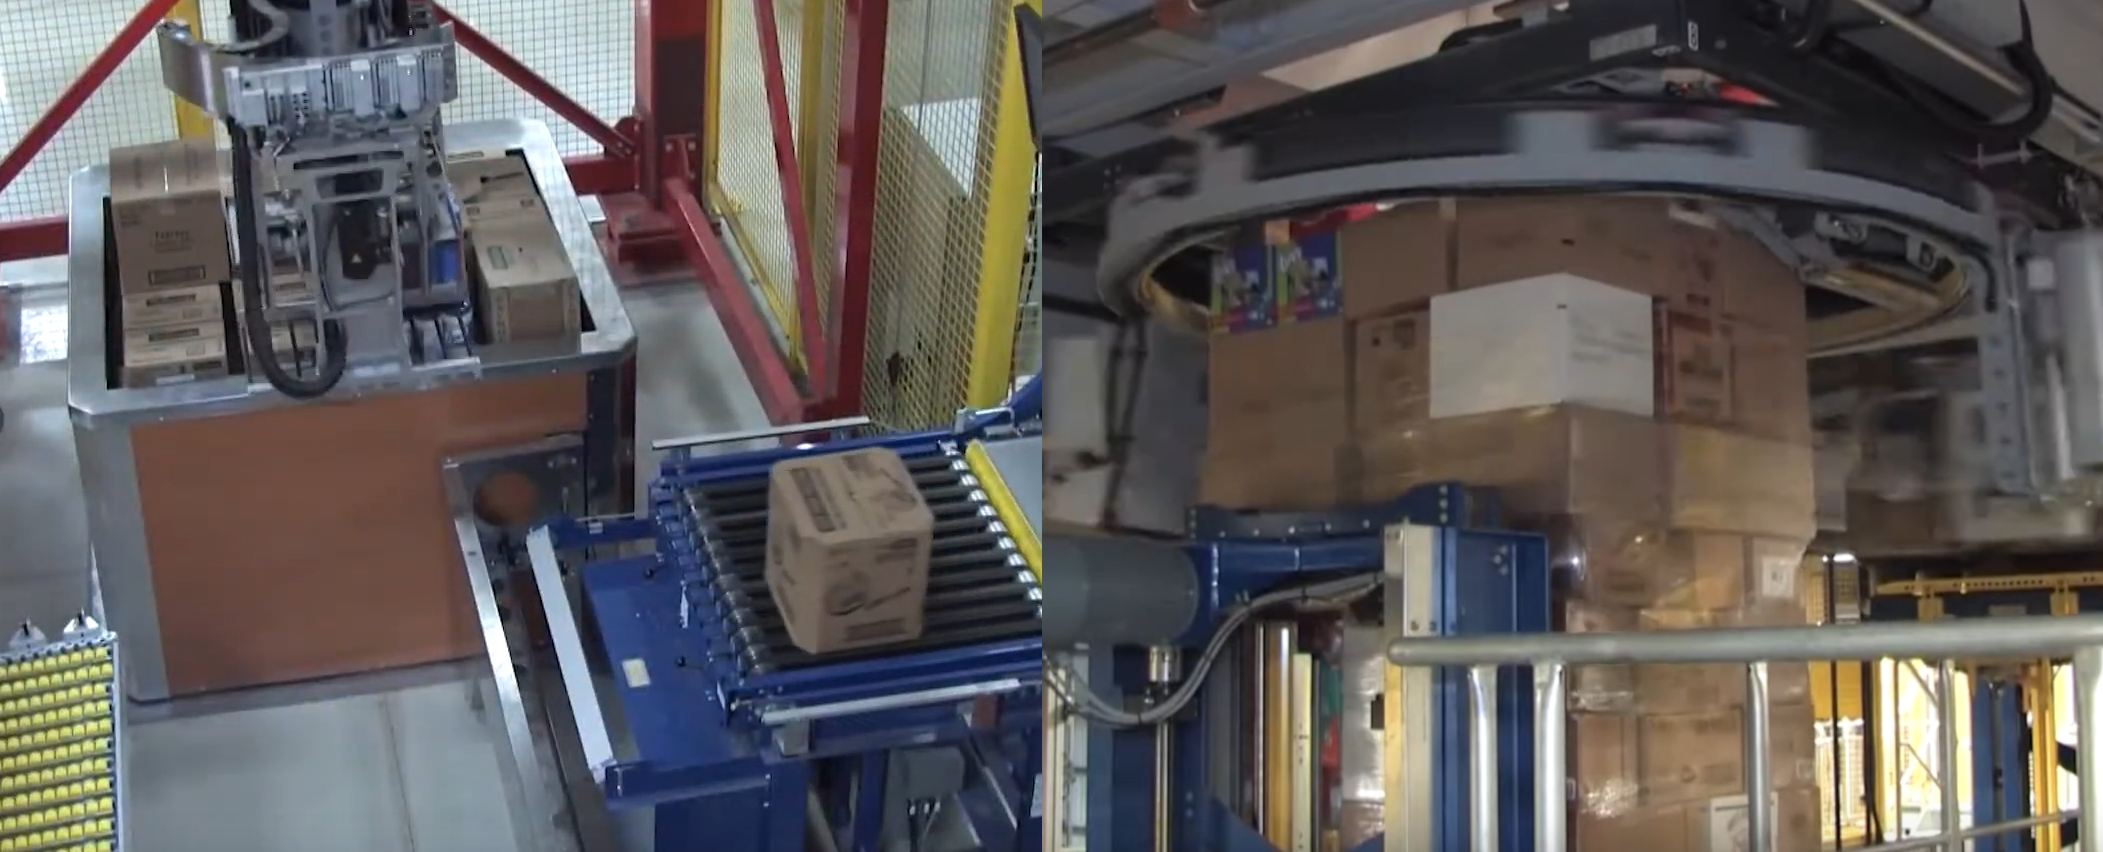
\includegraphics{Images/presentation/example_pit_pallettization.png}
                    }
                    \caption{Example of pit pallettization (\hyperlink{https://www.youtube.com/watch?v=_sSdk1baNLA}{Schäfer Case Picking | SSI SCHÄFER})}
                \end{figure}
            \column{55mm}
                \begin{figure}
                    \resizebox{\columnwidth}{!}{%
                        
\includegraphics{Images/logo_ermesx_highcontrast}
                    }
                \end{figure}
                \begin{figure}
                    \resizebox{\columnwidth}{!}{%
                        

\tikzset{every picture/.style={line width=0.75pt}} %set default line width to 0.75pt        

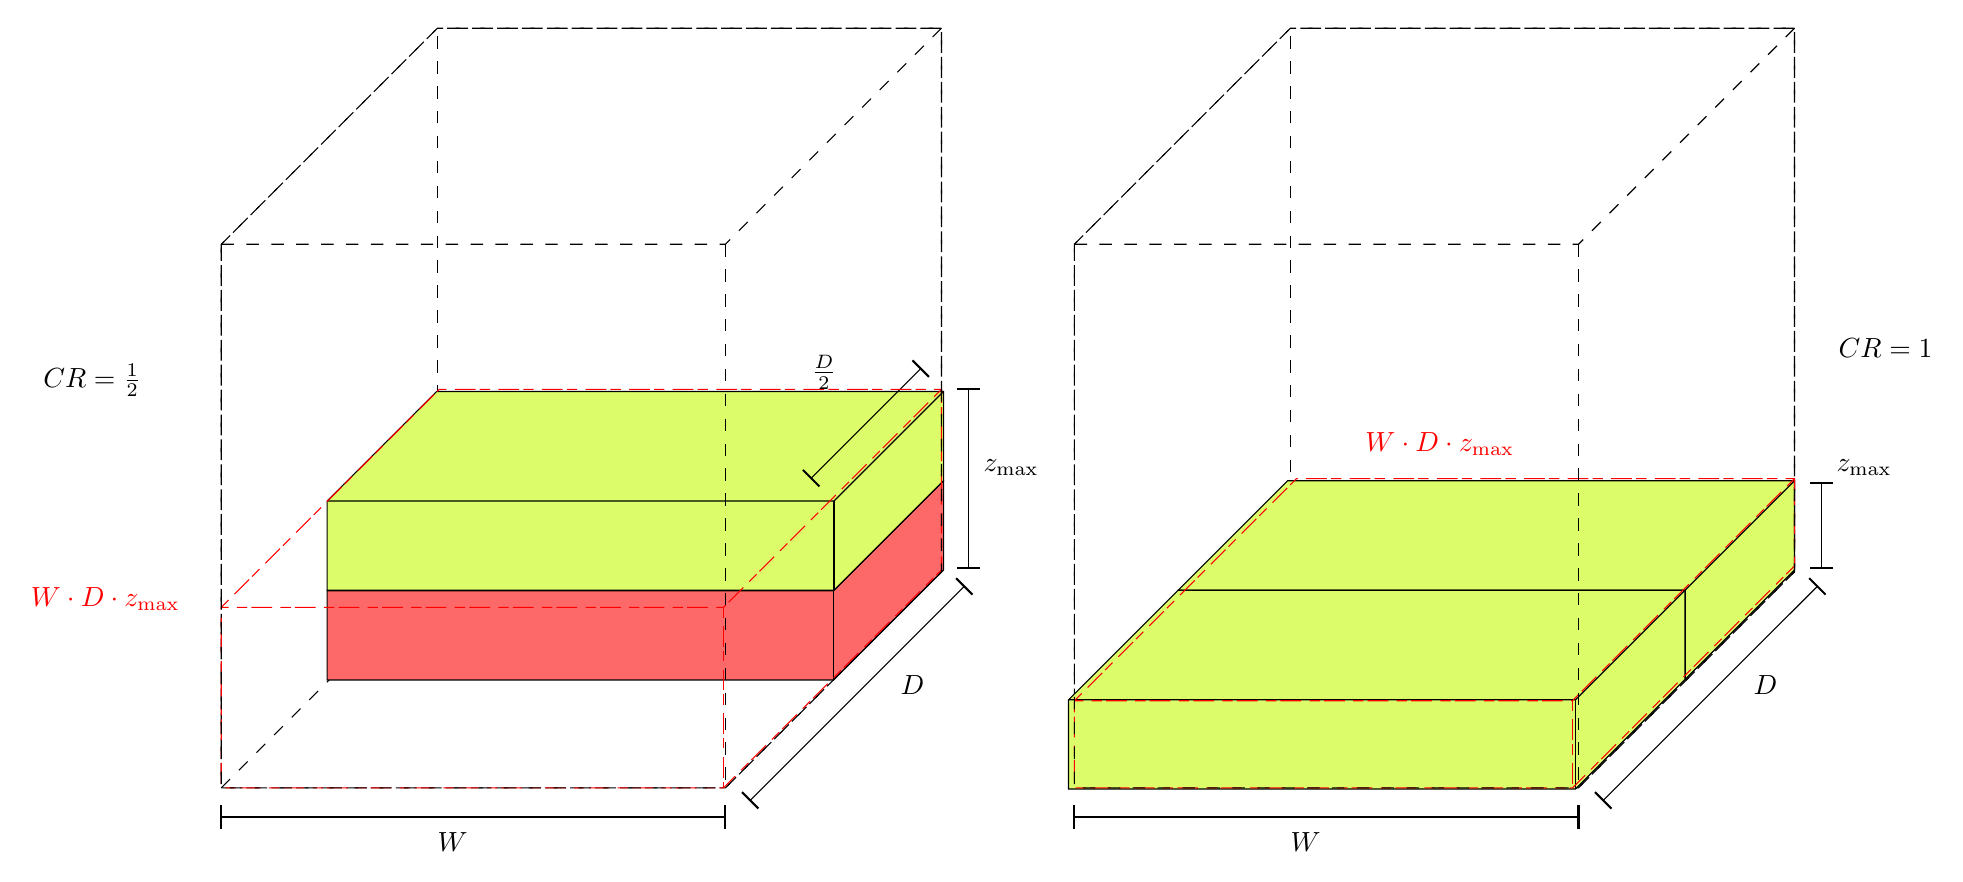
\begin{tikzpicture}[x=0.75pt,y=0.75pt,yscale=-1,xscale=1]
%uncomment if require: \path (0,479); %set diagram left start at 0, and has height of 479

%Shape: Cube [id:dp9446615397697055] 
\draw  [dash pattern={on 4.5pt off 4.5pt}] (917,301.9) -- (812.9,406) -- (570,406) -- (570,144.1) -- (674.1,40) -- (917,40) -- cycle ; \draw  [dash pattern={on 4.5pt off 4.5pt}] (570,406) -- (674.1,301.9) -- (917,301.9) ; \draw  [dash pattern={on 4.5pt off 4.5pt}] (674.1,301.9) -- (674.1,40) ;
%Shape: Cube [id:dp9924623151681093] 
\draw  [fill={rgb, 255:red, 220; green, 253; blue, 105 }  ,fill opacity=1 ] (620,310.78) -- (672.78,258) -- (917,258) -- (917,301) -- (864.22,353.78) -- (620,353.78) -- cycle ; \draw   (917,258) -- (864.22,310.78) -- (620,310.78) ; \draw   (864.22,310.78) -- (864.22,353.78) ;
%Shape: Cube [id:dp4356357707795666] 
\draw  [fill={rgb, 255:red, 220; green, 253; blue, 105 }  ,fill opacity=1 ] (567.22,363.56) -- (620,310.78) -- (864.22,310.78) -- (864.22,353.78) -- (811.44,406.56) -- (567.22,406.56) -- cycle ; \draw   (864.22,310.78) -- (811.44,363.56) -- (567.22,363.56) ; \draw   (811.44,363.56) -- (811.44,406.56) ;
%Shape: Cube [id:dp900981008021689] 
\draw  [dash pattern={on 4.5pt off 4.5pt}] (506,301.9) -- (401.9,406) -- (159,406) -- (159,144.1) -- (263.1,40) -- (506,40) -- cycle ; \draw  [dash pattern={on 4.5pt off 4.5pt}] (159,406) -- (263.1,301.9) -- (506,301.9) ; \draw  [dash pattern={on 4.5pt off 4.5pt}] (263.1,301.9) -- (263.1,40) ;
%Shape: Cube [id:dp9462720863667783] 
\draw  [fill={rgb, 255:red, 253; green, 105; blue, 105 }  ,fill opacity=1 ] (210,311) -- (263,258) -- (507,258) -- (507,301) -- (454,354) -- (210,354) -- cycle ; \draw   (507,258) -- (454,311) -- (210,311) ; \draw   (454,311) -- (454,354) ;
%Shape: Cube [id:dp20686523528460465] 
\draw  [fill={rgb, 255:red, 220; green, 253; blue, 105 }  ,fill opacity=1 ] (210,267.78) -- (262.78,215) -- (507,215) -- (507,258) -- (454.22,310.78) -- (210,310.78) -- cycle ; \draw   (507,215) -- (454.22,267.78) -- (210,267.78) ; \draw   (454.22,267.78) -- (454.22,310.78) ;
%Straight Lines [id:da9583369995131138] 
\draw    (496,204) -- (443.22,256.78) ;
\draw [shift={(443.22,256.78)}, rotate = 315] [color={rgb, 255:red, 0; green, 0; blue, 0 }  ][line width=0.75]    (0,5.59) -- (0,-5.59)   ;
\draw [shift={(496,204)}, rotate = 315] [color={rgb, 255:red, 0; green, 0; blue, 0 }  ][line width=0.75]    (0,5.59) -- (0,-5.59)   ;
%Straight Lines [id:da4480701288134522] 
\draw    (401.9,420) -- (159,420) ;
\draw [shift={(159,420)}, rotate = 360] [color={rgb, 255:red, 0; green, 0; blue, 0 }  ][line width=0.75]    (0,5.59) -- (0,-5.59)   ;
\draw [shift={(401.9,420)}, rotate = 360] [color={rgb, 255:red, 0; green, 0; blue, 0 }  ][line width=0.75]    (0,5.59) -- (0,-5.59)   ;
%Straight Lines [id:da9761873387202039] 
\draw    (517,308.9) -- (413.86,412) ;
\draw [shift={(413.86,412)}, rotate = 315.01] [color={rgb, 255:red, 0; green, 0; blue, 0 }  ][line width=0.75]    (0,5.59) -- (0,-5.59)   ;
\draw [shift={(517,308.9)}, rotate = 315.01] [color={rgb, 255:red, 0; green, 0; blue, 0 }  ][line width=0.75]    (0,5.59) -- (0,-5.59)   ;
%Straight Lines [id:da1211437330301477] 
\draw    (519,214) -- (519,299.86) ;
\draw [shift={(519,299.86)}, rotate = 270] [color={rgb, 255:red, 0; green, 0; blue, 0 }  ][line width=0.75]    (0,5.59) -- (0,-5.59)   ;
\draw [shift={(519,214)}, rotate = 270] [color={rgb, 255:red, 0; green, 0; blue, 0 }  ][line width=0.75]    (0,5.59) -- (0,-5.59)   ;
%Shape: Cube [id:dp6016430781165488] 
\draw  [color={rgb, 255:red, 255; green, 0; blue, 0 }  ,draw opacity=1 ][dash pattern={on 3.75pt off 3pt on 7.5pt off 1.5pt}] (159,319) -- (264,214) -- (506,214) -- (506,301) -- (401,406) -- (159,406) -- cycle ; \draw  [color={rgb, 255:red, 255; green, 0; blue, 0 }  ,draw opacity=1 ][dash pattern={on 3.75pt off 3pt on 7.5pt off 1.5pt}] (506,214) -- (401,319) -- (159,319) ; \draw  [color={rgb, 255:red, 255; green, 0; blue, 0 }  ,draw opacity=1 ][dash pattern={on 3.75pt off 3pt on 7.5pt off 1.5pt}] (401,319) -- (401,406) ;
%Shape: Cube [id:dp9858212525551202] 
\draw  [dash pattern={on 4.5pt off 4.5pt}] (159,144.1) -- (263.1,40) -- (506,40) -- (506,301.9) -- (401.9,406) -- (159,406) -- cycle ; \draw  [dash pattern={on 4.5pt off 4.5pt}] (506,40) -- (401.9,144.1) -- (159,144.1) ; \draw  [dash pattern={on 4.5pt off 4.5pt}] (401.9,144.1) -- (401.9,406) ;
%Straight Lines [id:da4537070040642701] 
\draw    (812.9,420) -- (570,420) ;
\draw [shift={(570,420)}, rotate = 360] [color={rgb, 255:red, 0; green, 0; blue, 0 }  ][line width=0.75]    (0,5.59) -- (0,-5.59)   ;
\draw [shift={(812.9,420)}, rotate = 360] [color={rgb, 255:red, 0; green, 0; blue, 0 }  ][line width=0.75]    (0,5.59) -- (0,-5.59)   ;
%Straight Lines [id:da13051427322471099] 
\draw    (928,308.9) -- (824.86,412) ;
\draw [shift={(824.86,412)}, rotate = 315.01] [color={rgb, 255:red, 0; green, 0; blue, 0 }  ][line width=0.75]    (0,5.59) -- (0,-5.59)   ;
\draw [shift={(928,308.9)}, rotate = 315.01] [color={rgb, 255:red, 0; green, 0; blue, 0 }  ][line width=0.75]    (0,5.59) -- (0,-5.59)   ;
%Straight Lines [id:da38828166025774113] 
\draw    (930,259) -- (930,299.86) ;
\draw [shift={(930,299.86)}, rotate = 270] [color={rgb, 255:red, 0; green, 0; blue, 0 }  ][line width=0.75]    (0,5.59) -- (0,-5.59)   ;
\draw [shift={(930,259)}, rotate = 270] [color={rgb, 255:red, 0; green, 0; blue, 0 }  ][line width=0.75]    (0,5.59) -- (0,-5.59)   ;
%Shape: Cube [id:dp33203292048167843] 
\draw  [color={rgb, 255:red, 255; green, 0; blue, 0 }  ,draw opacity=1 ][dash pattern={on 3.75pt off 3pt on 7.5pt off 1.5pt}] (570,364) -- (677,257) -- (917,257) -- (917,299) -- (810,406) -- (570,406) -- cycle ; \draw  [color={rgb, 255:red, 255; green, 0; blue, 0 }  ,draw opacity=1 ][dash pattern={on 3.75pt off 3pt on 7.5pt off 1.5pt}] (917,257) -- (810,364) -- (570,364) ; \draw  [color={rgb, 255:red, 255; green, 0; blue, 0 }  ,draw opacity=1 ][dash pattern={on 3.75pt off 3pt on 7.5pt off 1.5pt}] (810,364) -- (810,406) ;
%Shape: Cube [id:dp6959350788468752] 
\draw  [dash pattern={on 4.5pt off 4.5pt}] (570,144.1) -- (674.1,40) -- (917,40) -- (917,301.9) -- (812.9,406) -- (570,406) -- cycle ; \draw  [dash pattern={on 4.5pt off 4.5pt}] (917,40) -- (812.9,144.1) -- (570,144.1) ; \draw  [dash pattern={on 4.5pt off 4.5pt}] (812.9,144.1) -- (812.9,406) ;

% Text Node
\draw (442,196.4) node [anchor=north west][inner sep=0.75pt]    {$\frac{D}{2}$};
% Text Node
\draw (262,426.4) node [anchor=north west][inner sep=0.75pt]    {$W$};
% Text Node
\draw (485,350.4) node [anchor=north west][inner sep=0.75pt]    {$D$};
% Text Node
\draw (72,200.4) node [anchor=north west][inner sep=0.75pt]    {$CR=\frac{1}{2}$};
% Text Node
\draw (525,246.4) node [anchor=north west][inner sep=0.75pt]    {$z_{\text{max}}$};
% Text Node
\draw (66,308.4) node [anchor=north west][inner sep=0.75pt]  [color={rgb, 255:red, 255; green, 0; blue, 0 }  ,opacity=1 ]  {$W\cdot D\cdot z_{\text{max}}$};
% Text Node
\draw (673,426.4) node [anchor=north west][inner sep=0.75pt]    {$W$};
% Text Node
\draw (896,350.4) node [anchor=north west][inner sep=0.75pt]    {$D$};
% Text Node
\draw (937,188.4) node [anchor=north west][inner sep=0.75pt]    {$CR=1$};
% Text Node
\draw (936,246.4) node [anchor=north west][inner sep=0.75pt]    {$z_{\text{max}}$};
% Text Node
\draw (709,233.4) node [anchor=north west][inner sep=0.75pt]  [color={rgb, 255:red, 255; green, 0; blue, 0 }  ,opacity=1 ]  {$W\cdot D\cdot z_{\text{max}}$};


\end{tikzpicture}

                    }
                    \caption{Cage ratio of two different bin configurations}
                    \label{fig:cage_ratio}
                \end{figure}
        \end{columns}
    \end{frame}

    \begin{frame}{Vertical Support}
        \begin{block}{Definition}
            An item has vertical support if one of the following conditions hold:
            \begin{itemize}
                \item \textbf{Condition 1}: at least a percentage $\alpha_s$ of its base area is resting on other items
                \item \textbf{Condition 2}: at least 3 of its vertices are resting over other items and \textbf{Condition 1} holds with a lower percentage
            \end{itemize}
        \end{block}
    \end{frame}



    \begin{frame}{Vertical Support}
        \begin{figure}[H]
            \resizebox{\columnwidth}{!}{%
                

\tikzset{every picture/.style={line width=0.75pt}} %set default line width to 0.75pt        

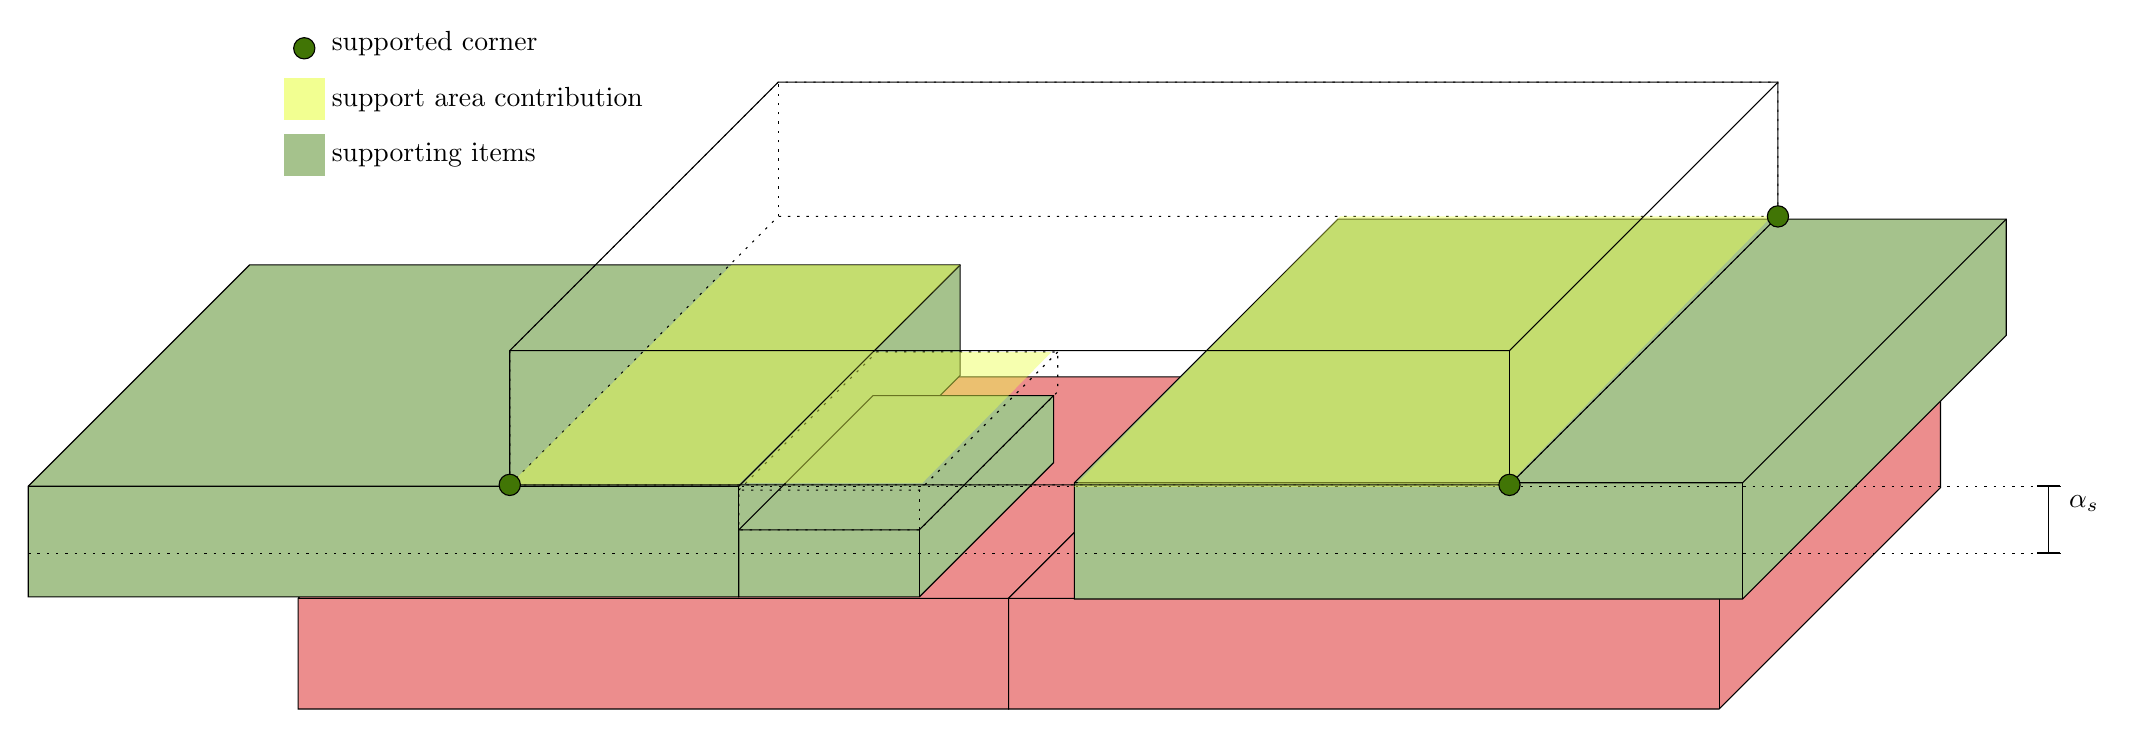
\begin{tikzpicture}[x=0.75pt,y=0.75pt,yscale=-1,xscale=1]
%uncomment if require: \path (0,479); %set diagram left start at 0, and has height of 479

%Shape: Cube [id:dp9411979483763162] 
\draw  [fill={rgb, 255:red, 236; green, 141; blue, 141 }  ,fill opacity=1 ] (194,306.67) -- (300.67,200) -- (643,200) -- (643,253.33) -- (536.33,360) -- (194,360) -- cycle ; \draw   (643,200) -- (536.33,306.67) -- (194,306.67) ; \draw   (536.33,306.67) -- (536.33,360) ;
%Shape: Cube [id:dp993645103603593] 
\draw  [fill={rgb, 255:red, 236; green, 141; blue, 141 }  ,fill opacity=1 ] (536.33,306.67) -- (643,200) -- (985.33,200) -- (985.33,253.33) -- (878.67,360) -- (536.33,360) -- cycle ; \draw   (985.33,200) -- (878.67,306.67) -- (536.33,306.67) ; \draw   (878.67,306.67) -- (878.67,360) ;
%Shape: Cube [id:dp23986673546182513] 
\draw  [fill={rgb, 255:red, 165; green, 194; blue, 140 }  ,fill opacity=1 ] (64,252.67) -- (170.67,146) -- (513,146) -- (513,199.33) -- (406.33,306) -- (64,306) -- cycle ; \draw   (513,146) -- (406.33,252.67) -- (64,252.67) ; \draw   (406.33,252.67) -- (406.33,306) ;
%Shape: Cube [id:dp5474008601617114] 
\draw  [fill={rgb, 255:red, 165; green, 194; blue, 140 }  ,fill opacity=1 ] (406.33,273.67) -- (471,209) -- (558,209) -- (558,241.33) -- (493.33,306) -- (406.33,306) -- cycle ; \draw   (558,209) -- (493.33,273.67) -- (406.33,273.67) ; \draw   (493.33,273.67) -- (493.33,306) ;
%Shape: Cube [id:dp7313777533771082] 
\draw  [fill={rgb, 255:red, 165; green, 194; blue, 140 }  ,fill opacity=1 ] (568,251) -- (695,124) -- (1017,124) -- (1017,180) -- (890,307) -- (568,307) -- cycle ; \draw   (1017,124) -- (890,251) -- (568,251) ; \draw   (890,251) -- (890,307) ;
%Shape: Cube [id:dp9978562503762016] 
\draw  [dash pattern={on 0.84pt off 2.51pt}] (907,122.67) -- (777.67,252) -- (296,252) -- (296,187.33) -- (425.33,58) -- (907,58) -- cycle ; \draw  [dash pattern={on 0.84pt off 2.51pt}] (296,252) -- (425.33,122.67) -- (907,122.67) ; \draw  [dash pattern={on 0.84pt off 2.51pt}] (425.33,122.67) -- (425.33,58) ;
%Shape: Cube [id:dp48964002783685845] 
\draw  [color={rgb, 255:red, 0; green, 0; blue, 0 }  ,draw opacity=1 ][fill={rgb, 255:red, 255; green, 255; blue, 255 }  ,fill opacity=0 ][dash pattern={on 0.84pt off 2.51pt}] (406.33,254.53) -- (472.86,188) -- (560,188) -- (560,207.14) -- (493.47,273.67) -- (406.33,273.67) -- cycle ; \draw  [color={rgb, 255:red, 0; green, 0; blue, 0 }  ,draw opacity=1 ][dash pattern={on 0.84pt off 2.51pt}] (560,188) -- (493.47,254.53) -- (406.33,254.53) ; \draw  [color={rgb, 255:red, 0; green, 0; blue, 0 }  ,draw opacity=1 ][dash pattern={on 0.84pt off 2.51pt}] (493.47,254.53) -- (493.47,273.67) ;
%Straight Lines [id:da26590658600836115] 
\draw    (1037.33,252.67) -- (1037.33,285) ;
\draw [shift={(1037.33,285)}, rotate = 270] [color={rgb, 255:red, 0; green, 0; blue, 0 }  ][line width=0.75]    (0,5.59) -- (0,-5.59)   ;
\draw [shift={(1037.33,252.67)}, rotate = 270] [color={rgb, 255:red, 0; green, 0; blue, 0 }  ][line width=0.75]    (0,5.59) -- (0,-5.59)   ;
%Straight Lines [id:da8302030012021052] 
\draw  [dash pattern={on 0.84pt off 2.51pt}]  (64,285) -- (1044,285) ;
%Straight Lines [id:da5354149137938202] 
\draw  [dash pattern={on 0.84pt off 2.51pt}]  (64,252.67) -- (1044,252.67) ;
%Shape: Parallelogram [id:dp4597753988697182] 
\draw  [color={rgb, 255:red, 0; green, 0; blue, 0 }  ,draw opacity=0 ][fill={rgb, 255:red, 234; green, 255; blue, 77 }  ,fill opacity=0.45 ] (403,146) -- (513,146) -- (406,252) -- (296,252) -- cycle ;
%Shape: Parallelogram [id:dp9407100355043312] 
\draw  [color={rgb, 255:red, 0; green, 0; blue, 0 }  ,draw opacity=0 ][fill={rgb, 255:red, 234; green, 255; blue, 77 }  ,fill opacity=0.45 ] (471,188) -- (557,188) -- (494.86,251) -- (408.86,251) -- cycle ;
%Shape: Parallelogram [id:dp5499917231467685] 
\draw  [color={rgb, 255:red, 0; green, 0; blue, 0 }  ,draw opacity=0 ][fill={rgb, 255:red, 234; green, 255; blue, 77 }  ,fill opacity=0.45 ] (696,122.67) -- (904,122.67) -- (775.67,253) -- (567.67,253) -- cycle ;
%Shape: Cube [id:dp21506487392572304] 
\draw   (296,187.33) -- (425.33,58) -- (907,58) -- (907,122.67) -- (777.67,252) -- (296,252) -- cycle ; \draw   (907,58) -- (777.67,187.33) -- (296,187.33) ; \draw   (777.67,187.33) -- (777.67,252) ;
%Shape: Rectangle [id:dp8515603217170198] 
\draw  [color={rgb, 255:red, 0; green, 0; blue, 0 }  ,draw opacity=0 ][fill={rgb, 255:red, 234; green, 255; blue, 77 }  ,fill opacity=0.62 ] (187,56) -- (207,56) -- (207,76) -- (187,76) -- cycle ;
%Shape: Rectangle [id:dp8969674268045522] 
\draw  [color={rgb, 255:red, 0; green, 0; blue, 0 }  ,draw opacity=0 ][fill={rgb, 255:red, 165; green, 194; blue, 140 }  ,fill opacity=1 ] (187,83) -- (207,83) -- (207,103) -- (187,103) -- cycle ;
%Shape: Circle [id:dp08410160878408413] 
\draw  [fill={rgb, 255:red, 65; green, 117; blue, 5 }  ,fill opacity=1 ] (290.88,252) .. controls (290.88,249.17) and (293.17,246.88) .. (296,246.88) .. controls (298.83,246.88) and (301.13,249.17) .. (301.13,252) .. controls (301.13,254.83) and (298.83,257.13) .. (296,257.13) .. controls (293.17,257.13) and (290.88,254.83) .. (290.88,252) -- cycle ;
%Shape: Circle [id:dp20799682119759832] 
\draw  [fill={rgb, 255:red, 65; green, 117; blue, 5 }  ,fill opacity=1 ] (772.54,252) .. controls (772.54,249.17) and (774.84,246.88) .. (777.67,246.88) .. controls (780.5,246.88) and (782.79,249.17) .. (782.79,252) .. controls (782.79,254.83) and (780.5,257.13) .. (777.67,257.13) .. controls (774.84,257.13) and (772.54,254.83) .. (772.54,252) -- cycle ;
%Shape: Circle [id:dp9242580914559287] 
\draw  [fill={rgb, 255:red, 65; green, 117; blue, 5 }  ,fill opacity=1 ] (901.88,122.67) .. controls (901.88,119.84) and (904.17,117.54) .. (907,117.54) .. controls (909.83,117.54) and (912.13,119.84) .. (912.13,122.67) .. controls (912.13,125.5) and (909.83,127.79) .. (907,127.79) .. controls (904.17,127.79) and (901.88,125.5) .. (901.88,122.67) -- cycle ;
%Shape: Circle [id:dp40386474009325335] 
\draw  [fill={rgb, 255:red, 65; green, 117; blue, 5 }  ,fill opacity=1 ] (191.88,41.67) .. controls (191.88,38.84) and (194.17,36.54) .. (197,36.54) .. controls (199.83,36.54) and (202.13,38.84) .. (202.13,41.67) .. controls (202.13,44.5) and (199.83,46.79) .. (197,46.79) .. controls (194.17,46.79) and (191.88,44.5) .. (191.88,41.67) -- cycle ;

% Text Node
\draw (1046,256.07) node [anchor=north west][inner sep=0.75pt]    {$\alpha _{s}$};
% Text Node
\draw (209,59) node [anchor=north west][inner sep=0.75pt]   [align=left] {support area contribution};
% Text Node
\draw (209,86) node [anchor=north west][inner sep=0.75pt]   [align=left] {supporting items};
% Text Node
\draw (209,32) node [anchor=north west][inner sep=0.75pt]   [align=left] {supported corner};


\end{tikzpicture}

            }
            \caption{Representation of an item with conditions 1 and 2 of vertical support given $\alpha_s = 0.5, \beta_s$}
            \label{fig:support}
        \end{figure}
    \end{frame}

    \section{Problem Definition}
    \begin{frame}{Literature Review}
        %TODO: Images for placement strategies
        \begin{itemize}
            \item The problem is NP-Hard
            \item Exact methods only for small instances %Cite?
            \item Existing 3D-BPP heuristics don't consider practical constraints
            \item Solutions for container loading and pallet loading problems are layer based
        \end{itemize}
    \end{frame}

    \begin{frame}{Conceptual Formulation}
        \begin{eqnarray*}
            \textbf{minimize} & \text{number of used bins} \\
            \textbf{then, maximize} & \text{average cage ratio of the used bins} \\
            \textbf{subject to} & \text{all items are assigned to one and only one bin} \\
                                              & \text{all items are inside the bin's bounds} \\
                                              & \text{no overlaps between items in the same bin} \\
                                              & \text{all items have vertical support} \\
        \end{eqnarray*}
    \end{frame}

    \begin{frame}{MILP Proxy Model - Objective Function}

        \begin{columns}[onlytextwidth,T]
            \column{\dimexpr\linewidth-75mm-5mm}
                \vspace{.25\textheight}
                \resizebox{13mm}{!}{
                    \begin{minipage}{\linewidth}
                    \begin{eqnarray*}
                        \textbf{minimize} & \text{number of used bins} \\
                        \textbf{then, maximize} & \text{average cage ratio of the used bins} \\
                        \color{gray}
                        \textbf{subject to} & \color{gray} \text{all items are assigned to one and only one bin} \\
                                                            & \color{gray} \text{all items are inside the bin's bounds} \\
                                                            & \color{gray} \text{no overlaps between items in the same bin} \\
                                                            & \color{gray} \text{all items have vertical support} \\
                    \end{eqnarray*}
                    \end{minipage}
                }

            \column{75mm}
            \resizebox{!}{30mm}{
                \begin{minipage}{\linewidth}
                    \begin{align}
                       \min       \qquad& \sum\limits_{b \in B} (H v_b + z^{max}_b) & \notag \\
                      \text{s.t.} \qquad & \color{gray} \sum\limits_{b \in B} u_{ib} + \sum\limits_{b \in B} u_{jb} = 1                          & \color{gray} \forall (i, j) \in I^{OR} \notag \\
                                         & \color{gray} u_{ib} \le v_b                                                                           & \color{gray} \forall i \in I, \forall b \in B \notag \\
                                         & \color{gray} v_b \ge v_c                                                                              & \color{gray} \forall (b,c) \in B : b < c  \notag \\
                                         & \color{gray} x_i + w_i \le W                                                                          & \color{gray} \forall i \in I \notag \\ 
                                         & \color{gray} y_i + d_i \le D                                                                          & \color{gray} \forall i \in I \notag \\ 
                                         & \color{gray} z_i + h_i \le H                                                                          & \color{gray} \forall i \in I \notag \\ 
                                         & \color{gray} (x_i + w_i) - x_j\le W(1 - x^p_{ij})                                                     & \color{gray} \forall i,j \in I \notag \\
                                         & \color{gray} x_j - (x_i + w_i) + 1 \le W x^p_{ij}                                                     & \color{gray} \forall i,j \in I \notag \\
                                         & \color{gray} (y_i + d_i) - y_j \le D(1 - y^p_{ij})                                                    & \color{gray} \forall i,j \in I \notag \\
                                         & \color{gray} y_j - (y_i + d_i) + 1 \le D y^p_{ij}                                                     & \color{gray} \forall i,j \in I \notag \\
                                         & \color{gray} (z_i + h_i) - z_j\le H(1 - z^p_{ij})                                                     & \color{gray} \forall i,j \in I \notag \\
                                         & \color{gray} z_j - (z_i + h_i) + 1 \le H z^p_{ij}                                                     & \color{gray} \forall i,j \in I \notag \\
                                         & \color{gray} x^p_{ij} + x^p_{ji} + y^p_{ij} + y^p_{ji} + z^p_{ij} + z^p_{ji} \ge u_{ib} + u_{jb} - 1  & \color{gray} \forall i,j \in I, \forall b \in B \notag \\
                                         & z^{max}_b \ge (z_i + h_i) - H(1-u_{ib})                                                               & \forall i \in I, \forall b \in B \notag
                    \end{align}
                \end{minipage}
            }
            \end{columns}
    \end{frame}

    \begin{frame}{MILP Proxy Model - Geometric Constraints 1}

        \begin{columns}[onlytextwidth,T]
            \column{\dimexpr\linewidth-75mm-5mm}
                \vspace{.25\textheight}
                \resizebox{13mm}{!}{
                    \begin{minipage}{\linewidth}
                    \begin{eqnarray*}
                        \color{gray} \textbf{minimize} & \color{gray} \text{number of used bins} \\
                        \color{gray} \textbf{then, maximize} & \color{gray} \text{average cage ratio of the used bins} \\
                        \textbf{subject to} & \text{all items are assigned to one and only one bin} \\
                                                            & \color{gray} \text{all items are inside the bin's bounds} \\
                                                            & \color{gray} \text{no overlaps between items in the same bin} \\
                                                            & \color{gray} \text{all items have vertical support} \\
                    \end{eqnarray*}
                    \end{minipage}
                }

            \column{75mm}
            \resizebox{!}{30mm}{
                \begin{minipage}{\linewidth}
                    \begin{align}
                \color{gray} \min \qquad & \color{gray} \sum\limits_{b \in B} (H v_b + z^{max}_b)                                                & \notag \\
                      \text{s.t.} \qquad & \sum\limits_{b \in B} u_{ib} + \sum\limits_{b \in B} u_{jb} = 1                          & \forall (i, j) \in I^{OR} \notag \\
                                         & u_{ib} \le v_b                                                                           & \forall i \in I, \forall b \in B \notag \\
                                         & v_b \ge v_c                                                                              & \forall (b,c) \in B : b < c  \notag \\
                                         & \color{gray} x_i + w_i \le W                                                                          & \color{gray} \forall i \in I \notag \\ 
                                         & \color{gray} y_i + d_i \le D                                                                          & \color{gray} \forall i \in I \notag \\ 
                                         & \color{gray} z_i + h_i \le H                                                                          & \color{gray} \forall i \in I \notag \\ 
                                         & \color{gray} (x_i + w_i) - x_j\le W(1 - x^p_{ij})                                                     & \color{gray} \forall i,j \in I \notag \\
                                         & \color{gray} x_j - (x_i + w_i) + 1 \le W x^p_{ij}                                                     & \color{gray} \forall i,j \in I \notag \\
                                         & \color{gray} (y_i + d_i) - y_j \le D(1 - y^p_{ij})                                                    & \color{gray} \forall i,j \in I \notag \\
                                         & \color{gray} y_j - (y_i + d_i) + 1 \le D y^p_{ij}                                                     & \color{gray} \forall i,j \in I \notag \\
                                         & \color{gray} (z_i + h_i) - z_j\le H(1 - z^p_{ij})                                                     & \color{gray} \forall i,j \in I \notag \\
                                         & \color{gray} z_j - (z_i + h_i) + 1 \le H z^p_{ij}                                                     & \color{gray} \forall i,j \in I \notag \\
                                         & \color{gray} x^p_{ij} + x^p_{ji} + y^p_{ij} + y^p_{ji} + z^p_{ij} + z^p_{ji} \ge u_{ib} + u_{jb} - 1  & \color{gray} \forall i,j \in I, \forall b \in B \notag \\
                                         & \color{gray} z^{max}_b \ge (z_i + h_i) - H(1-u_{ib})                                                  & \color{gray} \forall i \in I, \forall b \in B \notag
                    \end{align}
                \end{minipage}
            }
            \end{columns}
    \end{frame}


    \begin{frame}{MILP Proxy Model - Geometric Constraints 2}

        \begin{columns}[onlytextwidth,T]
            \column{\dimexpr\linewidth-75mm-5mm}
                \vspace{.25\textheight}
                \resizebox{13mm}{!}{
                    \begin{minipage}{\linewidth}
                    \begin{eqnarray*}
                        \color{gray} \textbf{minimize} & \color{gray} \text{number of used bins} \\
                        \color{gray} \textbf{then, maximize} & \color{gray} \text{average cage ratio of the used bins} \\
                        \textbf{subject to} & \color{gray} \text{all items are assigned to one and only one bin} \\
                                                            & \text{all items are inside the bin's bounds} \\
                                                            & \color{gray} \text{no overlaps between items in the same bin} \\
                                                            & \color{gray} \text{all items have vertical support} \\
                    \end{eqnarray*}
                    \end{minipage}
                }

            \column{75mm}
            \resizebox{!}{30mm}{
                \begin{minipage}{\linewidth}
                    \begin{align}
                \color{gray} \min \qquad & \color{gray} \sum\limits_{b \in B} (H v_b + z^{max}_b)                                                & \notag \\
                      \text{s.t.} \qquad & \color{gray} \sum\limits_{b \in B} u_{ib} + \sum\limits_{b \in B} u_{jb} = 1                          & \color{gray} \forall (i, j) \in I^{OR} \notag \\
                                         & \color{gray} u_{ib} \le v_b                                                                           & \color{gray} \forall i \in I, \forall b \in B \notag \\
                                         & \color{gray} v_b \ge v_c                                                                              & \color{gray} \forall (b,c) \in B : b < c  \notag \\
                                         & x_i + w_i \le W                                                                          & \forall i \in I \notag \\ 
                                         & y_i + d_i \le D                                                                          & \forall i \in I \notag \\ 
                                         & z_i + h_i \le H                                                                          & \forall i \in I \notag \\ 
                                         & \color{gray} (x_i + w_i) - x_j\le W(1 - x^p_{ij})                                                     & \color{gray} \forall i,j \in I \notag \\
                                         & \color{gray} x_j - (x_i + w_i) + 1 \le W x^p_{ij}                                                     & \color{gray} \forall i,j \in I \notag \\
                                         & \color{gray} (y_i + d_i) - y_j \le D(1 - y^p_{ij})                                                    & \color{gray} \forall i,j \in I \notag \\
                                         & \color{gray} y_j - (y_i + d_i) + 1 \le D y^p_{ij}                                                     & \color{gray} \forall i,j \in I \notag \\
                                         & \color{gray} (z_i + h_i) - z_j\le H(1 - z^p_{ij})                                                     & \color{gray} \forall i,j \in I \notag \\
                                         & \color{gray} z_j - (z_i + h_i) + 1 \le H z^p_{ij}                                                     & \color{gray} \forall i,j \in I \notag \\
                                         & \color{gray} x^p_{ij} + x^p_{ji} + y^p_{ij} + y^p_{ji} + z^p_{ij} + z^p_{ji} \ge u_{ib} + u_{jb} - 1  & \color{gray} \forall i,j \in I, \forall b \in B \notag \\
                                         & \color{gray} z^{max}_b \ge (z_i + h_i) - H(1-u_{ib})                                                  & \color{gray} \forall i \in I, \forall b \in B \notag
                    \end{align}
                \end{minipage}
            }
            \end{columns}
    \end{frame}


    \begin{frame}{MILP Proxy Model - Geometric Constraints 3}

        \begin{columns}[onlytextwidth,T]
            \column{\dimexpr\linewidth-75mm-5mm}
                \vspace{.12\textheight}
                \resizebox{13mm}{!}{
                    \begin{minipage}{\linewidth}
                    \begin{eqnarray*}
                        \color{gray} \textbf{minimize} & \color{gray} \text{number of used bins} \\
                        \color{gray} \textbf{then, maximize} & \color{gray} \text{average cage ratio of the used bins} \\
                        \textbf{subject to} & \color{gray} \text{all items are assigned to one and only one bin} \\
                                                            & \color{gray} \text{all items are inside the bin's bounds} \\
                                                            & \text{no overlaps between items in the same bin} \\
                                                            & \color{gray} \text{all items have vertical support} \\
                    \end{eqnarray*}
                    \end{minipage}
                }
                
                \begin{figure}
                    \resizebox{1.35\columnwidth}{!}{
                        

\tikzset{every picture/.style={line width=0.75pt}} %set default line width to 0.75pt        

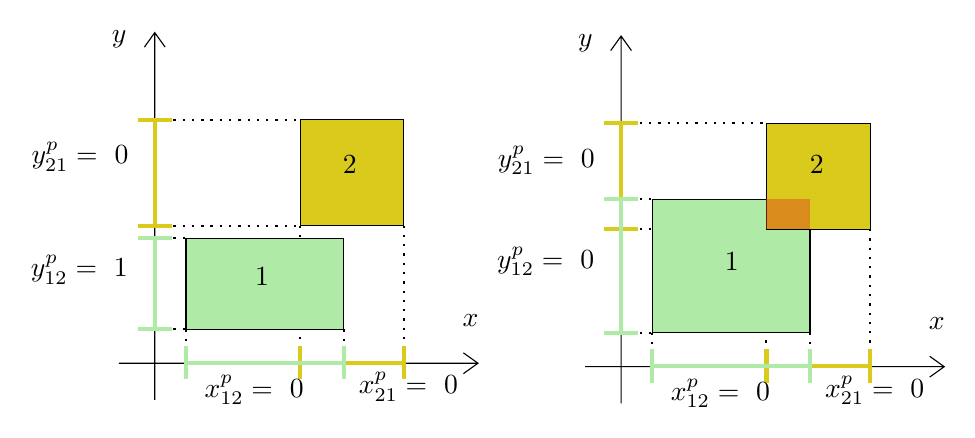
\begin{tikzpicture}[x=0.75pt,y=0.75pt,yscale=-1,xscale=1]
%uncomment if require: \path (0,300); %set diagram left start at 0, and has height of 300

%Straight Lines [id:da16944613342131554] 
\draw [color={rgb, 255:red, 0; green, 0; blue, 0 }  ,draw opacity=1 ][line width=0.75]  [dash pattern={on 0.84pt off 2.51pt}]  (77,247.5) -- (77,263.5) ;
%Straight Lines [id:da32247408153225543] 
\draw [color={rgb, 255:red, 0; green, 0; blue, 0 }  ,draw opacity=1 ][line width=0.75]  [dash pattern={on 0.84pt off 2.51pt}]  (153,247.5) -- (153,263.5) ;
%Straight Lines [id:da39889490826632257] 
\draw [color={rgb, 255:red, 0; green, 0; blue, 0 }  ,draw opacity=1 ][line width=0.75]  [dash pattern={on 0.84pt off 2.51pt}]  (182,197.5) -- (182,263.5) ;
%Straight Lines [id:da7240587122118071] 
\draw [color={rgb, 255:red, 0; green, 0; blue, 0 }  ,draw opacity=1 ][line width=0.75]  [dash pattern={on 0.84pt off 2.51pt}]  (132,197.5) -- (132,263.5) ;
%Straight Lines [id:da4848715482257471] 
\draw [color={rgb, 255:red, 0; green, 0; blue, 0 }  ,draw opacity=1 ][line width=0.75]  [dash pattern={on 0.84pt off 2.51pt}]  (62,247.5) -- (77,247.5) ;
%Straight Lines [id:da4670272012004465] 
\draw [color={rgb, 255:red, 0; green, 0; blue, 0 }  ,draw opacity=1 ][line width=0.75]  [dash pattern={on 0.84pt off 2.51pt}]  (62,203.5) -- (77,203.5) ;
%Straight Lines [id:da7178245871900936] 
\draw [color={rgb, 255:red, 0; green, 0; blue, 0 }  ,draw opacity=1 ][line width=0.75]  [dash pattern={on 0.84pt off 2.51pt}]  (62,197.5) -- (132,197.5) ;
%Straight Lines [id:da3847931225791108] 
\draw [color={rgb, 255:red, 0; green, 0; blue, 0 }  ,draw opacity=1 ][line width=0.75]  [dash pattern={on 0.84pt off 2.51pt}]  (62,146.5) -- (132,146.5) ;
%Shape: Rectangle [id:dp49230539255936656] 
\draw  [fill={rgb, 255:red, 175; green, 235; blue, 167 }  ,fill opacity=1 ] (77,203.5) -- (153,203.5) -- (153,247.5) -- (77,247.5) -- cycle ;
%Shape: Axis 2D [id:dp7101905015075989] 
\draw  (44.67,263.8) -- (217.67,263.8)(61.97,104.5) -- (61.97,281.5) (210.67,258.8) -- (217.67,263.8) -- (210.67,268.8) (56.97,111.5) -- (61.97,104.5) -- (66.97,111.5)  ;
%Shape: Rectangle [id:dp7631610956479798] 
\draw  [fill={rgb, 255:red, 217; green, 202; blue, 28 }  ,fill opacity=1 ] (132,146.5) -- (182,146.5) -- (182,197.5) -- (132,197.5) -- cycle ;
%Straight Lines [id:da5582007065184471] 
\draw [color={rgb, 255:red, 217; green, 202; blue, 28 }  ,draw opacity=1 ][line width=1.5]    (62,146.5) -- (62,197.5) ;
\draw [shift={(62,197.5)}, rotate = 270] [color={rgb, 255:red, 217; green, 202; blue, 28 }  ,draw opacity=1 ][line width=1.5]    (0,8.05) -- (0,-8.05)   ;
\draw [shift={(62,146.5)}, rotate = 270] [color={rgb, 255:red, 217; green, 202; blue, 28 }  ,draw opacity=1 ][line width=1.5]    (0,8.05) -- (0,-8.05)   ;
%Straight Lines [id:da4131577420929736] 
\draw [color={rgb, 255:red, 175; green, 235; blue, 167 }  ,draw opacity=1 ][line width=1.5]    (62,203.5) -- (62,247.5) ;
\draw [shift={(62,247.5)}, rotate = 270] [color={rgb, 255:red, 175; green, 235; blue, 167 }  ,draw opacity=1 ][line width=1.5]    (0,8.05) -- (0,-8.05)   ;
\draw [shift={(62,203.5)}, rotate = 270] [color={rgb, 255:red, 175; green, 235; blue, 167 }  ,draw opacity=1 ][line width=1.5]    (0,8.05) -- (0,-8.05)   ;
%Straight Lines [id:da9955798074260177] 
\draw [color={rgb, 255:red, 217; green, 202; blue, 28 }  ,draw opacity=1 ][line width=1.5]    (182,263.5) -- (132,263.5) ;
\draw [shift={(132,263.5)}, rotate = 360] [color={rgb, 255:red, 217; green, 202; blue, 28 }  ,draw opacity=1 ][line width=1.5]    (0,8.05) -- (0,-8.05)   ;
\draw [shift={(182,263.5)}, rotate = 360] [color={rgb, 255:red, 217; green, 202; blue, 28 }  ,draw opacity=1 ][line width=1.5]    (0,8.05) -- (0,-8.05)   ;
%Straight Lines [id:da8846703181763751] 
\draw [color={rgb, 255:red, 175; green, 235; blue, 167 }  ,draw opacity=1 ][line width=1.5]    (153,263.5) -- (77,263.5) ;
\draw [shift={(77,263.5)}, rotate = 360] [color={rgb, 255:red, 175; green, 235; blue, 167 }  ,draw opacity=1 ][line width=1.5]    (0,8.05) -- (0,-8.05)   ;
\draw [shift={(153,263.5)}, rotate = 360] [color={rgb, 255:red, 175; green, 235; blue, 167 }  ,draw opacity=1 ][line width=1.5]    (0,8.05) -- (0,-8.05)   ;
%Straight Lines [id:da49719565576066305] 
\draw [color={rgb, 255:red, 0; green, 0; blue, 0 }  ,draw opacity=1 ][line width=0.75]  [dash pattern={on 0.84pt off 2.51pt}]  (301.67,249.17) -- (301.67,265.17) ;
%Straight Lines [id:da9307804167194788] 
\draw [color={rgb, 255:red, 0; green, 0; blue, 0 }  ,draw opacity=1 ][line width=0.75]  [dash pattern={on 0.84pt off 2.51pt}]  (377.67,249.17) -- (377.67,265.17) ;
%Straight Lines [id:da8413555856997723] 
\draw [color={rgb, 255:red, 0; green, 0; blue, 0 }  ,draw opacity=1 ][line width=0.75]  [dash pattern={on 0.84pt off 2.51pt}]  (406.67,199.17) -- (406.67,265.17) ;
%Straight Lines [id:da10291713605161046] 
\draw [color={rgb, 255:red, 0; green, 0; blue, 0 }  ,draw opacity=1 ][line width=0.75]  [dash pattern={on 0.84pt off 2.51pt}]  (356.67,199.17) -- (356.67,265.17) ;
%Straight Lines [id:da07228496188863687] 
\draw [color={rgb, 255:red, 0; green, 0; blue, 0 }  ,draw opacity=1 ][line width=0.75]  [dash pattern={on 0.84pt off 2.51pt}]  (286.67,249.17) -- (301.67,249.17) ;
%Straight Lines [id:da46264525124314493] 
\draw [color={rgb, 255:red, 0; green, 0; blue, 0 }  ,draw opacity=1 ][line width=0.75]  [dash pattern={on 0.84pt off 2.51pt}]  (286.67,184.83) -- (301.67,184.83) ;
%Straight Lines [id:da10518295101301789] 
\draw [color={rgb, 255:red, 0; green, 0; blue, 0 }  ,draw opacity=1 ][line width=0.75]  [dash pattern={on 0.84pt off 2.51pt}]  (286.67,199.17) -- (356.67,199.17) ;
%Straight Lines [id:da48759903920739567] 
\draw [color={rgb, 255:red, 0; green, 0; blue, 0 }  ,draw opacity=1 ][line width=0.75]  [dash pattern={on 0.84pt off 2.51pt}]  (286.67,148.17) -- (356.67,148.17) ;
%Shape: Rectangle [id:dp8428401541536165] 
\draw  [fill={rgb, 255:red, 175; green, 235; blue, 167 }  ,fill opacity=1 ] (301.67,184.83) -- (377.67,184.83) -- (377.67,249.17) -- (301.67,249.17) -- cycle ;
%Shape: Axis 2D [id:dp5220394057294739] 
\draw  (269.33,265.47) -- (442.33,265.47)(286.63,106.17) -- (286.63,283.17) (435.33,260.47) -- (442.33,265.47) -- (435.33,270.47) (281.63,113.17) -- (286.63,106.17) -- (291.63,113.17)  ;
%Shape: Rectangle [id:dp0753512868890468] 
\draw  [fill={rgb, 255:red, 217; green, 202; blue, 28 }  ,fill opacity=1 ] (356.67,148.17) -- (406.67,148.17) -- (406.67,199.17) -- (356.67,199.17) -- cycle ;
%Straight Lines [id:da4893768766826617] 
\draw [color={rgb, 255:red, 217; green, 202; blue, 28 }  ,draw opacity=1 ][line width=1.5]    (286.67,148.17) -- (286.67,199.17) ;
\draw [shift={(286.67,199.17)}, rotate = 270] [color={rgb, 255:red, 217; green, 202; blue, 28 }  ,draw opacity=1 ][line width=1.5]    (0,8.05) -- (0,-8.05)   ;
\draw [shift={(286.67,148.17)}, rotate = 270] [color={rgb, 255:red, 217; green, 202; blue, 28 }  ,draw opacity=1 ][line width=1.5]    (0,8.05) -- (0,-8.05)   ;
%Straight Lines [id:da004775269316056874] 
\draw [color={rgb, 255:red, 175; green, 235; blue, 167 }  ,draw opacity=1 ][line width=1.5]    (286.67,184.83) -- (286.67,249.17) ;
\draw [shift={(286.67,249.17)}, rotate = 270] [color={rgb, 255:red, 175; green, 235; blue, 167 }  ,draw opacity=1 ][line width=1.5]    (0,8.05) -- (0,-8.05)   ;
\draw [shift={(286.67,184.83)}, rotate = 270] [color={rgb, 255:red, 175; green, 235; blue, 167 }  ,draw opacity=1 ][line width=1.5]    (0,8.05) -- (0,-8.05)   ;
%Straight Lines [id:da7258310112961572] 
\draw [color={rgb, 255:red, 217; green, 202; blue, 28 }  ,draw opacity=1 ][line width=1.5]    (406.67,265.17) -- (356.67,265.17) ;
\draw [shift={(356.67,265.17)}, rotate = 360] [color={rgb, 255:red, 217; green, 202; blue, 28 }  ,draw opacity=1 ][line width=1.5]    (0,8.05) -- (0,-8.05)   ;
\draw [shift={(406.67,265.17)}, rotate = 360] [color={rgb, 255:red, 217; green, 202; blue, 28 }  ,draw opacity=1 ][line width=1.5]    (0,8.05) -- (0,-8.05)   ;
%Straight Lines [id:da32809815226067063] 
\draw [color={rgb, 255:red, 175; green, 235; blue, 167 }  ,draw opacity=1 ][line width=1.5]    (377.67,265.17) -- (301.67,265.17) ;
\draw [shift={(301.67,265.17)}, rotate = 360] [color={rgb, 255:red, 175; green, 235; blue, 167 }  ,draw opacity=1 ][line width=1.5]    (0,8.05) -- (0,-8.05)   ;
\draw [shift={(377.67,265.17)}, rotate = 360] [color={rgb, 255:red, 175; green, 235; blue, 167 }  ,draw opacity=1 ][line width=1.5]    (0,8.05) -- (0,-8.05)   ;
%Shape: Rectangle [id:dp3980152579597326] 
\draw  [draw opacity=0][fill={rgb, 255:red, 217; green, 68; blue, 28 }  ,fill opacity=0.46 ] (356.67,184.83) -- (377.67,184.83) -- (377.67,199.17) -- (356.67,199.17) -- cycle ;

% Text Node
\draw (1,210.4) node [anchor=north west][inner sep=0.75pt]    {$y_{12}^{p} =\ 1$};
% Text Node
\draw (1.33,156.07) node [anchor=north west][inner sep=0.75pt]    {$y_{21}^{p} =\ 0$};
% Text Node
\draw (159,266.9) node [anchor=north west][inner sep=0.75pt]    {$x_{21}^{p} =\ 0$};
% Text Node
\draw (84.67,268.4) node [anchor=north west][inner sep=0.75pt]    {$x_{12}^{p} =\ 0$};
% Text Node
\draw (209,239.07) node [anchor=north west][inner sep=0.75pt]    {$x$};
% Text Node
\draw (40,102.4) node [anchor=north west][inner sep=0.75pt]    {$y$};
% Text Node
\draw (225.67,206.4) node [anchor=north west][inner sep=0.75pt]    {$y_{12}^{p} =\ 0$};
% Text Node
\draw (226,157.73) node [anchor=north west][inner sep=0.75pt]    {$y_{21}^{p} =\ 0$};
% Text Node
\draw (383.67,268.57) node [anchor=north west][inner sep=0.75pt]    {$x_{21}^{p} =\ 0$};
% Text Node
\draw (309.33,270.07) node [anchor=north west][inner sep=0.75pt]    {$x_{12}^{p} =\ 0$};
% Text Node
\draw (433.67,240.73) node [anchor=north west][inner sep=0.75pt]    {$x$};
% Text Node
\draw (264.67,104.07) node [anchor=north west][inner sep=0.75pt]    {$y$};
% Text Node
\draw (109,216.4) node [anchor=north west][inner sep=0.75pt]    {$1$};
% Text Node
\draw (151.33,162.4) node [anchor=north west][inner sep=0.75pt]    {$2$};
% Text Node
\draw (335.33,209.07) node [anchor=north west][inner sep=0.75pt]    {$1$};
% Text Node
\draw (376.33,162.4) node [anchor=north west][inner sep=0.75pt]    {$2$};


\end{tikzpicture}

                    }
                    \caption{Precedences variables (2D case)}
                \end{figure}
            \column{75mm}
            \resizebox{!}{30mm}{
                \begin{minipage}{\linewidth}
                    \begin{align}
                \color{gray} \min \qquad & \color{gray} \sum\limits_{b \in B} (H v_b + z^{max}_b)                                                & \notag \\
                      \text{s.t.} \qquad & \color{gray} \sum\limits_{b \in B} u_{ib} + \sum\limits_{b \in B} u_{jb} = 1                          & \color{gray} \forall (i, j) \in I^{OR} \notag \\
                                         & \color{gray} u_{ib} \le v_b                                                                           & \color{gray} \forall i \in I, \forall b \in B \notag \\
                                         & \color{gray} v_b \ge v_c                                                                              & \color{gray} \forall (b,c) \in B : b < c  \notag \\
                                         & \color{gray} x_i + w_i \le W                                                                          & \color{gray} \forall i \in I \notag \\ 
                                         & \color{gray} y_i + d_i \le D                                                                          & \color{gray} \forall i \in I \notag \\ 
                                         & \color{gray} z_i + h_i \le H                                                                          & \color{gray} \forall i \in I \notag \\ 
                                         & (x_i + w_i) - x_j\le W(1 - x^p_{ij})                                                     & \forall i,j \in I \notag \\
                                         & x_j - (x_i + w_i) + 1 \le W x^p_{ij}                                                     & \forall i,j \in I \notag \\
                                         & (y_i + d_i) - y_j \le D(1 - y^p_{ij})                                                    & \forall i,j \in I \notag \\
                                         & y_j - (y_i + d_i) + 1 \le D y^p_{ij}                                                     & \forall i,j \in I \notag \\
                                         & (z_i + h_i) - z_j\le H(1 - z^p_{ij})                                                     & \forall i,j \in I \notag \\
                                         & z_j - (z_i + h_i) + 1 \le H z^p_{ij}                                                     & \forall i,j \in I \notag \\
                                         & x^p_{ij} + x^p_{ji} + y^p_{ij} + y^p_{ji} + z^p_{ij} + z^p_{ji} \ge u_{ib} + u_{jb} - 1  & \forall i,j \in I, \forall b \in B \notag \\
                                         & \color{gray} z^{max}_b \ge (z_i + h_i) - H(1-u_{ib})                                                  & \color{gray} \forall i \in I, \forall b \in B \notag
                    \end{align}
                \end{minipage}
            }
            \end{columns}
    \end{frame}

    \begin{frame}{MILP Proxy Model - Discretized Vertical Support}


        \begin{columns}[onlytextwidth,T]
            \column{\dimexpr\linewidth-75mm-5mm}
                \vspace{.12\textheight}
                \resizebox{13mm}{!}{
                    \begin{minipage}{\linewidth}
                    \begin{eqnarray*}
                        \color{gray} \textbf{minimize} & \color{gray} \text{number of used bins} \\
                        \color{gray} \textbf{then, maximize} & \color{gray} \text{average cage ratio of the used bins} \\
                        \textbf{subject to} & \color{gray} \text{all items are assigned to one and only one bin} \\
                                                            & \color{gray} \text{all items are inside the bin's bounds} \\
                                                            & \color{gray} \text{no overlaps between items in the same bin} \\
                                                            & \text{all items have vertical support} \\
                    \end{eqnarray*}
                    \end{minipage}
                }
                \vspace{-5mm}
                \begin{figure}
                    \hspace*{-5mm}
                    \resizebox{1.35\columnwidth}{!}{
                        

\tikzset{every picture/.style={line width=0.75pt}} %set default line width to 0.75pt        

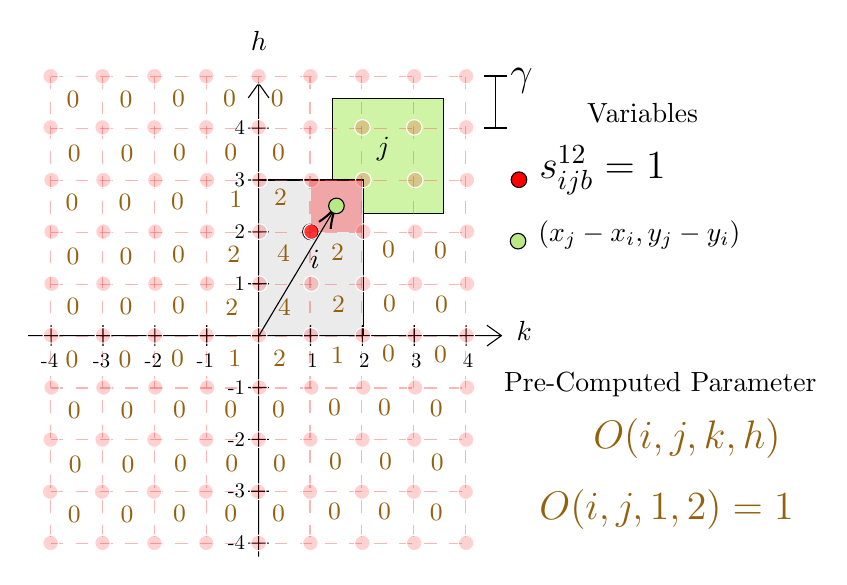
\begin{tikzpicture}[x=0.75pt,y=0.75pt,yscale=-1,xscale=1]
%uncomment if require: \path (0,300); %set diagram left start at 0, and has height of 300

%Shape: Rectangle [id:dp5959662237650998] 
\draw  [color={rgb, 255:red, 0; green, 0; blue, 0 }  ,draw opacity=1 ][fill={rgb, 255:red, 207; green, 244; blue, 165 }  ,fill opacity=1 ] (167.5,47.25) -- (221,47.25) -- (221,102.75) -- (167.5,102.75) -- cycle ;
%Shape: Rectangle [id:dp3153208771996219] 
\draw  [fill={rgb, 255:red, 235; green, 235; blue, 235 }  ,fill opacity=1 ] (132,86.5) -- (182.44,86.5) -- (182.44,161.5) -- (132,161.5) -- cycle ;
%Shape: Grid [id:dp3665057478133332] 
\draw  [draw opacity=0][fill={rgb, 255:red, 0; green, 0; blue, 0 }  ,fill opacity=0 ][dash pattern={on 4.5pt off 4.5pt}] (31.78,36.72) -- (232.78,36.72) -- (232.78,262.72) -- (31.78,262.72) -- cycle ; \draw  [color={rgb, 255:red, 247; green, 92; blue, 92 }  ,draw opacity=0.45 ][dash pattern={on 4.5pt off 4.5pt}] (31.78,36.72) -- (31.78,262.72)(56.78,36.72) -- (56.78,262.72)(81.78,36.72) -- (81.78,262.72)(106.78,36.72) -- (106.78,262.72)(131.78,36.72) -- (131.78,262.72)(156.78,36.72) -- (156.78,262.72)(181.78,36.72) -- (181.78,262.72)(206.78,36.72) -- (206.78,262.72)(231.78,36.72) -- (231.78,262.72) ; \draw  [color={rgb, 255:red, 247; green, 92; blue, 92 }  ,draw opacity=0.45 ][dash pattern={on 4.5pt off 4.5pt}] (31.78,36.72) -- (232.78,36.72)(31.78,61.72) -- (232.78,61.72)(31.78,86.72) -- (232.78,86.72)(31.78,111.72) -- (232.78,111.72)(31.78,136.72) -- (232.78,136.72)(31.78,161.72) -- (232.78,161.72)(31.78,186.72) -- (232.78,186.72)(31.78,211.72) -- (232.78,211.72)(31.78,236.72) -- (232.78,236.72)(31.78,261.72) -- (232.78,261.72) ; \draw  [color={rgb, 255:red, 247; green, 92; blue, 92 }  ,draw opacity=0.45 ][dash pattern={on 4.5pt off 4.5pt}]  ;
%Shape: Axis 2D [id:dp5870087683485721] 
\draw  (21,161.5) -- (249,161.5)(132,40) -- (132,268) (242,156.5) -- (249,161.5) -- (242,166.5) (127,47) -- (132,40) -- (137,47) (157,156.5) -- (157,166.5)(182,156.5) -- (182,166.5)(207,156.5) -- (207,166.5)(232,156.5) -- (232,166.5)(107,156.5) -- (107,166.5)(82,156.5) -- (82,166.5)(57,156.5) -- (57,166.5)(32,156.5) -- (32,166.5)(127,136.5) -- (137,136.5)(127,111.5) -- (137,111.5)(127,86.5) -- (137,86.5)(127,61.5) -- (137,61.5)(127,186.5) -- (137,186.5)(127,211.5) -- (137,211.5)(127,236.5) -- (137,236.5)(127,261.5) -- (137,261.5) ;
\draw   (164,173.5) node[anchor=east, scale=0.75]{1} (189,173.5) node[anchor=east, scale=0.75]{2} (214,173.5) node[anchor=east, scale=0.75]{3} (239,173.5) node[anchor=east, scale=0.75]{4} (114,173.5) node[anchor=east, scale=0.75]{-1} (89,173.5) node[anchor=east, scale=0.75]{-2} (64,173.5) node[anchor=east, scale=0.75]{-3} (39,173.5) node[anchor=east, scale=0.75]{-4} (129,136.5) node[anchor=east, scale=0.75]{1} (129,111.5) node[anchor=east, scale=0.75]{2} (129,86.5) node[anchor=east, scale=0.75]{3} (129,61.5) node[anchor=east, scale=0.75]{4} (129,186.5) node[anchor=east, scale=0.75]{-1} (129,211.5) node[anchor=east, scale=0.75]{-2} (129,236.5) node[anchor=east, scale=0.75]{-3} (129,261.5) node[anchor=east, scale=0.75]{-4} ;
%Straight Lines [id:da4474601658411276] 
\draw    (246,36.5) -- (246,61.5) ;
\draw [shift={(246,61.5)}, rotate = 270] [color={rgb, 255:red, 0; green, 0; blue, 0 }  ][line width=0.75]    (0,5.59) -- (0,-5.59)   ;
\draw [shift={(246,36.5)}, rotate = 270] [color={rgb, 255:red, 0; green, 0; blue, 0 }  ][line width=0.75]    (0,5.59) -- (0,-5.59)   ;
%Flowchart: Connector [id:dp17650433550879074] 
\draw  [color={rgb, 255:red, 255; green, 255; blue, 255 }  ,draw opacity=1 ][fill={rgb, 255:red, 255; green, 0; blue, 0 }  ,fill opacity=0.18 ] (28.03,36.5) .. controls (28.03,34.43) and (29.71,32.75) .. (31.78,32.75) .. controls (33.85,32.75) and (35.53,34.43) .. (35.53,36.5) .. controls (35.53,38.57) and (33.85,40.25) .. (31.78,40.25) .. controls (29.71,40.25) and (28.03,38.57) .. (28.03,36.5) -- cycle ;
%Flowchart: Connector [id:dp9770094792582217] 
\draw  [fill={rgb, 255:red, 255; green, 0; blue, 0 }  ,fill opacity=0.7 ] (153.25,111.5) .. controls (153.25,109.43) and (154.93,107.75) .. (157,107.75) .. controls (159.07,107.75) and (160.75,109.43) .. (160.75,111.5) .. controls (160.75,113.57) and (159.07,115.25) .. (157,115.25) .. controls (154.93,115.25) and (153.25,113.57) .. (153.25,111.5) -- cycle ;
%Flowchart: Connector [id:dp9315813149146155] 
\draw  [color={rgb, 255:red, 255; green, 255; blue, 255 }  ,draw opacity=1 ][fill={rgb, 255:red, 255; green, 0; blue, 0 }  ,fill opacity=0.18 ] (53.03,36.5) .. controls (53.03,34.43) and (54.71,32.75) .. (56.78,32.75) .. controls (58.85,32.75) and (60.53,34.43) .. (60.53,36.5) .. controls (60.53,38.57) and (58.85,40.25) .. (56.78,40.25) .. controls (54.71,40.25) and (53.03,38.57) .. (53.03,36.5) -- cycle ;
%Flowchart: Connector [id:dp8657956854954557] 
\draw  [color={rgb, 255:red, 255; green, 255; blue, 255 }  ,draw opacity=1 ][fill={rgb, 255:red, 255; green, 0; blue, 0 }  ,fill opacity=0.18 ] (78.03,36.5) .. controls (78.03,34.43) and (79.71,32.75) .. (81.78,32.75) .. controls (83.85,32.75) and (85.53,34.43) .. (85.53,36.5) .. controls (85.53,38.57) and (83.85,40.25) .. (81.78,40.25) .. controls (79.71,40.25) and (78.03,38.57) .. (78.03,36.5) -- cycle ;
%Flowchart: Connector [id:dp09342029252508777] 
\draw  [color={rgb, 255:red, 255; green, 255; blue, 255 }  ,draw opacity=1 ][fill={rgb, 255:red, 255; green, 0; blue, 0 }  ,fill opacity=0.18 ] (103.03,36.5) .. controls (103.03,34.43) and (104.71,32.75) .. (106.78,32.75) .. controls (108.85,32.75) and (110.53,34.43) .. (110.53,36.5) .. controls (110.53,38.57) and (108.85,40.25) .. (106.78,40.25) .. controls (104.71,40.25) and (103.03,38.57) .. (103.03,36.5) -- cycle ;
%Flowchart: Connector [id:dp533439523276273] 
\draw  [color={rgb, 255:red, 255; green, 255; blue, 255 }  ,draw opacity=1 ][fill={rgb, 255:red, 255; green, 0; blue, 0 }  ,fill opacity=0.18 ] (153.25,36.5) .. controls (153.25,34.43) and (154.93,32.75) .. (157,32.75) .. controls (159.07,32.75) and (160.75,34.43) .. (160.75,36.5) .. controls (160.75,38.57) and (159.07,40.25) .. (157,40.25) .. controls (154.93,40.25) and (153.25,38.57) .. (153.25,36.5) -- cycle ;
%Flowchart: Connector [id:dp17730485501604987] 
\draw  [color={rgb, 255:red, 255; green, 255; blue, 255 }  ,draw opacity=1 ][fill={rgb, 255:red, 255; green, 0; blue, 0 }  ,fill opacity=0.18 ] (178.25,36.5) .. controls (178.25,34.43) and (179.93,32.75) .. (182,32.75) .. controls (184.07,32.75) and (185.75,34.43) .. (185.75,36.5) .. controls (185.75,38.57) and (184.07,40.25) .. (182,40.25) .. controls (179.93,40.25) and (178.25,38.57) .. (178.25,36.5) -- cycle ;
%Flowchart: Connector [id:dp8819775226725283] 
\draw  [color={rgb, 255:red, 255; green, 255; blue, 255 }  ,draw opacity=1 ][fill={rgb, 255:red, 255; green, 0; blue, 0 }  ,fill opacity=0.18 ] (203.25,36.5) .. controls (203.25,34.43) and (204.93,32.75) .. (207,32.75) .. controls (209.07,32.75) and (210.75,34.43) .. (210.75,36.5) .. controls (210.75,38.57) and (209.07,40.25) .. (207,40.25) .. controls (204.93,40.25) and (203.25,38.57) .. (203.25,36.5) -- cycle ;
%Flowchart: Connector [id:dp1420881048740692] 
\draw  [color={rgb, 255:red, 255; green, 255; blue, 255 }  ,draw opacity=1 ][fill={rgb, 255:red, 255; green, 0; blue, 0 }  ,fill opacity=0.18 ] (228.25,36.5) .. controls (228.25,34.43) and (229.93,32.75) .. (232,32.75) .. controls (234.07,32.75) and (235.75,34.43) .. (235.75,36.5) .. controls (235.75,38.57) and (234.07,40.25) .. (232,40.25) .. controls (229.93,40.25) and (228.25,38.57) .. (228.25,36.5) -- cycle ;
%Flowchart: Connector [id:dp014549534119622898] 
\draw  [color={rgb, 255:red, 255; green, 255; blue, 255 }  ,draw opacity=1 ][fill={rgb, 255:red, 255; green, 0; blue, 0 }  ,fill opacity=0.18 ] (128.25,36.5) .. controls (128.25,34.43) and (129.93,32.75) .. (132,32.75) .. controls (134.07,32.75) and (135.75,34.43) .. (135.75,36.5) .. controls (135.75,38.57) and (134.07,40.25) .. (132,40.25) .. controls (129.93,40.25) and (128.25,38.57) .. (128.25,36.5) -- cycle ;
%Flowchart: Connector [id:dp5842977340969858] 
\draw  [color={rgb, 255:red, 255; green, 255; blue, 255 }  ,draw opacity=1 ][fill={rgb, 255:red, 255; green, 0; blue, 0 }  ,fill opacity=0.18 ] (28.03,61.17) .. controls (28.03,59.1) and (29.71,57.42) .. (31.78,57.42) .. controls (33.85,57.42) and (35.53,59.1) .. (35.53,61.17) .. controls (35.53,63.24) and (33.85,64.92) .. (31.78,64.92) .. controls (29.71,64.92) and (28.03,63.24) .. (28.03,61.17) -- cycle ;
%Flowchart: Connector [id:dp6519155112808065] 
\draw  [color={rgb, 255:red, 255; green, 255; blue, 255 }  ,draw opacity=1 ][fill={rgb, 255:red, 255; green, 0; blue, 0 }  ,fill opacity=0.18 ] (53.03,61.17) .. controls (53.03,59.1) and (54.71,57.42) .. (56.78,57.42) .. controls (58.85,57.42) and (60.53,59.1) .. (60.53,61.17) .. controls (60.53,63.24) and (58.85,64.92) .. (56.78,64.92) .. controls (54.71,64.92) and (53.03,63.24) .. (53.03,61.17) -- cycle ;
%Flowchart: Connector [id:dp36077536920560327] 
\draw  [color={rgb, 255:red, 255; green, 255; blue, 255 }  ,draw opacity=1 ][fill={rgb, 255:red, 255; green, 0; blue, 0 }  ,fill opacity=0.18 ] (78.03,61.17) .. controls (78.03,59.1) and (79.71,57.42) .. (81.78,57.42) .. controls (83.85,57.42) and (85.53,59.1) .. (85.53,61.17) .. controls (85.53,63.24) and (83.85,64.92) .. (81.78,64.92) .. controls (79.71,64.92) and (78.03,63.24) .. (78.03,61.17) -- cycle ;
%Flowchart: Connector [id:dp5189088045367096] 
\draw  [color={rgb, 255:red, 255; green, 255; blue, 255 }  ,draw opacity=1 ][fill={rgb, 255:red, 255; green, 0; blue, 0 }  ,fill opacity=0.18 ] (103.03,61.17) .. controls (103.03,59.1) and (104.71,57.42) .. (106.78,57.42) .. controls (108.85,57.42) and (110.53,59.1) .. (110.53,61.17) .. controls (110.53,63.24) and (108.85,64.92) .. (106.78,64.92) .. controls (104.71,64.92) and (103.03,63.24) .. (103.03,61.17) -- cycle ;
%Flowchart: Connector [id:dp05741768855482643] 
\draw  [color={rgb, 255:red, 255; green, 255; blue, 255 }  ,draw opacity=1 ][fill={rgb, 255:red, 255; green, 0; blue, 0 }  ,fill opacity=0.18 ] (153.25,61.17) .. controls (153.25,59.1) and (154.93,57.42) .. (157,57.42) .. controls (159.07,57.42) and (160.75,59.1) .. (160.75,61.17) .. controls (160.75,63.24) and (159.07,64.92) .. (157,64.92) .. controls (154.93,64.92) and (153.25,63.24) .. (153.25,61.17) -- cycle ;
%Flowchart: Connector [id:dp006363561960593622] 
\draw  [color={rgb, 255:red, 255; green, 255; blue, 255 }  ,draw opacity=1 ][fill={rgb, 255:red, 255; green, 0; blue, 0 }  ,fill opacity=0.18 ] (178.25,61.17) .. controls (178.25,59.1) and (179.93,57.42) .. (182,57.42) .. controls (184.07,57.42) and (185.75,59.1) .. (185.75,61.17) .. controls (185.75,63.24) and (184.07,64.92) .. (182,64.92) .. controls (179.93,64.92) and (178.25,63.24) .. (178.25,61.17) -- cycle ;
%Flowchart: Connector [id:dp46345859900758] 
\draw  [color={rgb, 255:red, 255; green, 255; blue, 255 }  ,draw opacity=1 ][fill={rgb, 255:red, 255; green, 0; blue, 0 }  ,fill opacity=0.18 ] (203.25,61.17) .. controls (203.25,59.1) and (204.93,57.42) .. (207,57.42) .. controls (209.07,57.42) and (210.75,59.1) .. (210.75,61.17) .. controls (210.75,63.24) and (209.07,64.92) .. (207,64.92) .. controls (204.93,64.92) and (203.25,63.24) .. (203.25,61.17) -- cycle ;
%Flowchart: Connector [id:dp019098380251666325] 
\draw  [color={rgb, 255:red, 255; green, 255; blue, 255 }  ,draw opacity=1 ][fill={rgb, 255:red, 255; green, 0; blue, 0 }  ,fill opacity=0.18 ] (228.25,61.17) .. controls (228.25,59.1) and (229.93,57.42) .. (232,57.42) .. controls (234.07,57.42) and (235.75,59.1) .. (235.75,61.17) .. controls (235.75,63.24) and (234.07,64.92) .. (232,64.92) .. controls (229.93,64.92) and (228.25,63.24) .. (228.25,61.17) -- cycle ;
%Flowchart: Connector [id:dp8272679894580149] 
\draw  [color={rgb, 255:red, 255; green, 255; blue, 255 }  ,draw opacity=1 ][fill={rgb, 255:red, 255; green, 0; blue, 0 }  ,fill opacity=0.18 ] (128.25,61.17) .. controls (128.25,59.1) and (129.93,57.42) .. (132,57.42) .. controls (134.07,57.42) and (135.75,59.1) .. (135.75,61.17) .. controls (135.75,63.24) and (134.07,64.92) .. (132,64.92) .. controls (129.93,64.92) and (128.25,63.24) .. (128.25,61.17) -- cycle ;
%Flowchart: Connector [id:dp01549254055562177] 
\draw  [color={rgb, 255:red, 255; green, 255; blue, 255 }  ,draw opacity=1 ][fill={rgb, 255:red, 255; green, 0; blue, 0 }  ,fill opacity=0.18 ] (28.47,86.5) .. controls (28.47,84.43) and (30.15,82.75) .. (32.22,82.75) .. controls (34.29,82.75) and (35.97,84.43) .. (35.97,86.5) .. controls (35.97,88.57) and (34.29,90.25) .. (32.22,90.25) .. controls (30.15,90.25) and (28.47,88.57) .. (28.47,86.5) -- cycle ;
%Flowchart: Connector [id:dp027166291716461677] 
\draw  [color={rgb, 255:red, 255; green, 255; blue, 255 }  ,draw opacity=1 ][fill={rgb, 255:red, 255; green, 0; blue, 0 }  ,fill opacity=0.18 ] (53.47,86.5) .. controls (53.47,84.43) and (55.15,82.75) .. (57.22,82.75) .. controls (59.29,82.75) and (60.97,84.43) .. (60.97,86.5) .. controls (60.97,88.57) and (59.29,90.25) .. (57.22,90.25) .. controls (55.15,90.25) and (53.47,88.57) .. (53.47,86.5) -- cycle ;
%Flowchart: Connector [id:dp8515274344244661] 
\draw  [color={rgb, 255:red, 255; green, 255; blue, 255 }  ,draw opacity=1 ][fill={rgb, 255:red, 255; green, 0; blue, 0 }  ,fill opacity=0.18 ] (78.47,86.5) .. controls (78.47,84.43) and (80.15,82.75) .. (82.22,82.75) .. controls (84.29,82.75) and (85.97,84.43) .. (85.97,86.5) .. controls (85.97,88.57) and (84.29,90.25) .. (82.22,90.25) .. controls (80.15,90.25) and (78.47,88.57) .. (78.47,86.5) -- cycle ;
%Flowchart: Connector [id:dp20327157268330664] 
\draw  [color={rgb, 255:red, 255; green, 255; blue, 255 }  ,draw opacity=1 ][fill={rgb, 255:red, 255; green, 0; blue, 0 }  ,fill opacity=0.18 ] (103.47,86.5) .. controls (103.47,84.43) and (105.15,82.75) .. (107.22,82.75) .. controls (109.29,82.75) and (110.97,84.43) .. (110.97,86.5) .. controls (110.97,88.57) and (109.29,90.25) .. (107.22,90.25) .. controls (105.15,90.25) and (103.47,88.57) .. (103.47,86.5) -- cycle ;
%Flowchart: Connector [id:dp13376132351948555] 
\draw  [color={rgb, 255:red, 255; green, 255; blue, 255 }  ,draw opacity=1 ][fill={rgb, 255:red, 255; green, 0; blue, 0 }  ,fill opacity=0.18 ] (153.69,86.5) .. controls (153.69,84.43) and (155.37,82.75) .. (157.44,82.75) .. controls (159.52,82.75) and (161.19,84.43) .. (161.19,86.5) .. controls (161.19,88.57) and (159.52,90.25) .. (157.44,90.25) .. controls (155.37,90.25) and (153.69,88.57) .. (153.69,86.5) -- cycle ;
%Flowchart: Connector [id:dp4044064224279934] 
\draw  [color={rgb, 255:red, 255; green, 255; blue, 255 }  ,draw opacity=1 ][fill={rgb, 255:red, 255; green, 0; blue, 0 }  ,fill opacity=0.18 ] (178.69,86.5) .. controls (178.69,84.43) and (180.37,82.75) .. (182.44,82.75) .. controls (184.52,82.75) and (186.19,84.43) .. (186.19,86.5) .. controls (186.19,88.57) and (184.52,90.25) .. (182.44,90.25) .. controls (180.37,90.25) and (178.69,88.57) .. (178.69,86.5) -- cycle ;
%Flowchart: Connector [id:dp07583386051229557] 
\draw  [color={rgb, 255:red, 255; green, 255; blue, 255 }  ,draw opacity=1 ][fill={rgb, 255:red, 255; green, 0; blue, 0 }  ,fill opacity=0.18 ] (203.69,86.5) .. controls (203.69,84.43) and (205.37,82.75) .. (207.44,82.75) .. controls (209.52,82.75) and (211.19,84.43) .. (211.19,86.5) .. controls (211.19,88.57) and (209.52,90.25) .. (207.44,90.25) .. controls (205.37,90.25) and (203.69,88.57) .. (203.69,86.5) -- cycle ;
%Flowchart: Connector [id:dp49124263363886067] 
\draw  [color={rgb, 255:red, 255; green, 255; blue, 255 }  ,draw opacity=1 ][fill={rgb, 255:red, 255; green, 0; blue, 0 }  ,fill opacity=0.18 ] (228.69,86.5) .. controls (228.69,84.43) and (230.37,82.75) .. (232.44,82.75) .. controls (234.52,82.75) and (236.19,84.43) .. (236.19,86.5) .. controls (236.19,88.57) and (234.52,90.25) .. (232.44,90.25) .. controls (230.37,90.25) and (228.69,88.57) .. (228.69,86.5) -- cycle ;
%Flowchart: Connector [id:dp8856760470116622] 
\draw  [color={rgb, 255:red, 255; green, 255; blue, 255 }  ,draw opacity=1 ][fill={rgb, 255:red, 255; green, 0; blue, 0 }  ,fill opacity=0.18 ] (128.69,86.5) .. controls (128.69,84.43) and (130.37,82.75) .. (132.44,82.75) .. controls (134.52,82.75) and (136.19,84.43) .. (136.19,86.5) .. controls (136.19,88.57) and (134.52,90.25) .. (132.44,90.25) .. controls (130.37,90.25) and (128.69,88.57) .. (128.69,86.5) -- cycle ;
%Flowchart: Connector [id:dp301207315319171] 
\draw  [color={rgb, 255:red, 255; green, 255; blue, 255 }  ,draw opacity=1 ][fill={rgb, 255:red, 255; green, 0; blue, 0 }  ,fill opacity=0.18 ] (28.47,111.39) .. controls (28.47,109.32) and (30.15,107.64) .. (32.22,107.64) .. controls (34.29,107.64) and (35.97,109.32) .. (35.97,111.39) .. controls (35.97,113.46) and (34.29,115.14) .. (32.22,115.14) .. controls (30.15,115.14) and (28.47,113.46) .. (28.47,111.39) -- cycle ;
%Flowchart: Connector [id:dp9873901030687902] 
\draw  [color={rgb, 255:red, 255; green, 255; blue, 255 }  ,draw opacity=1 ][fill={rgb, 255:red, 255; green, 0; blue, 0 }  ,fill opacity=0.18 ] (53.47,111.39) .. controls (53.47,109.32) and (55.15,107.64) .. (57.22,107.64) .. controls (59.29,107.64) and (60.97,109.32) .. (60.97,111.39) .. controls (60.97,113.46) and (59.29,115.14) .. (57.22,115.14) .. controls (55.15,115.14) and (53.47,113.46) .. (53.47,111.39) -- cycle ;
%Flowchart: Connector [id:dp5933980597190441] 
\draw  [color={rgb, 255:red, 255; green, 255; blue, 255 }  ,draw opacity=1 ][fill={rgb, 255:red, 255; green, 0; blue, 0 }  ,fill opacity=0.18 ] (78.47,111.39) .. controls (78.47,109.32) and (80.15,107.64) .. (82.22,107.64) .. controls (84.29,107.64) and (85.97,109.32) .. (85.97,111.39) .. controls (85.97,113.46) and (84.29,115.14) .. (82.22,115.14) .. controls (80.15,115.14) and (78.47,113.46) .. (78.47,111.39) -- cycle ;
%Flowchart: Connector [id:dp0845756744343803] 
\draw  [color={rgb, 255:red, 255; green, 255; blue, 255 }  ,draw opacity=1 ][fill={rgb, 255:red, 255; green, 0; blue, 0 }  ,fill opacity=0.18 ] (103.47,111.39) .. controls (103.47,109.32) and (105.15,107.64) .. (107.22,107.64) .. controls (109.29,107.64) and (110.97,109.32) .. (110.97,111.39) .. controls (110.97,113.46) and (109.29,115.14) .. (107.22,115.14) .. controls (105.15,115.14) and (103.47,113.46) .. (103.47,111.39) -- cycle ;
%Flowchart: Connector [id:dp29502546476584324] 
\draw  [color={rgb, 255:red, 255; green, 255; blue, 255 }  ,draw opacity=1 ][fill={rgb, 255:red, 255; green, 0; blue, 0 }  ,fill opacity=0.18 ] (153.69,111.39) .. controls (153.69,109.32) and (155.37,107.64) .. (157.44,107.64) .. controls (159.52,107.64) and (161.19,109.32) .. (161.19,111.39) .. controls (161.19,113.46) and (159.52,115.14) .. (157.44,115.14) .. controls (155.37,115.14) and (153.69,113.46) .. (153.69,111.39) -- cycle ;
%Flowchart: Connector [id:dp06874296669968716] 
\draw  [color={rgb, 255:red, 255; green, 255; blue, 255 }  ,draw opacity=1 ][fill={rgb, 255:red, 255; green, 0; blue, 0 }  ,fill opacity=0.18 ] (178.69,111.39) .. controls (178.69,109.32) and (180.37,107.64) .. (182.44,107.64) .. controls (184.52,107.64) and (186.19,109.32) .. (186.19,111.39) .. controls (186.19,113.46) and (184.52,115.14) .. (182.44,115.14) .. controls (180.37,115.14) and (178.69,113.46) .. (178.69,111.39) -- cycle ;
%Flowchart: Connector [id:dp9162544207566379] 
\draw  [color={rgb, 255:red, 255; green, 255; blue, 255 }  ,draw opacity=1 ][fill={rgb, 255:red, 255; green, 0; blue, 0 }  ,fill opacity=0.18 ] (203.69,111.39) .. controls (203.69,109.32) and (205.37,107.64) .. (207.44,107.64) .. controls (209.52,107.64) and (211.19,109.32) .. (211.19,111.39) .. controls (211.19,113.46) and (209.52,115.14) .. (207.44,115.14) .. controls (205.37,115.14) and (203.69,113.46) .. (203.69,111.39) -- cycle ;
%Flowchart: Connector [id:dp14989652582386304] 
\draw  [color={rgb, 255:red, 255; green, 255; blue, 255 }  ,draw opacity=1 ][fill={rgb, 255:red, 255; green, 0; blue, 0 }  ,fill opacity=0.18 ] (228.69,111.39) .. controls (228.69,109.32) and (230.37,107.64) .. (232.44,107.64) .. controls (234.52,107.64) and (236.19,109.32) .. (236.19,111.39) .. controls (236.19,113.46) and (234.52,115.14) .. (232.44,115.14) .. controls (230.37,115.14) and (228.69,113.46) .. (228.69,111.39) -- cycle ;
%Flowchart: Connector [id:dp3853078344508225] 
\draw  [color={rgb, 255:red, 255; green, 255; blue, 255 }  ,draw opacity=1 ][fill={rgb, 255:red, 255; green, 0; blue, 0 }  ,fill opacity=0.18 ] (128.69,111.39) .. controls (128.69,109.32) and (130.37,107.64) .. (132.44,107.64) .. controls (134.52,107.64) and (136.19,109.32) .. (136.19,111.39) .. controls (136.19,113.46) and (134.52,115.14) .. (132.44,115.14) .. controls (130.37,115.14) and (128.69,113.46) .. (128.69,111.39) -- cycle ;
%Flowchart: Connector [id:dp7343580941980375] 
\draw  [color={rgb, 255:red, 255; green, 255; blue, 255 }  ,draw opacity=1 ][fill={rgb, 255:red, 255; green, 0; blue, 0 }  ,fill opacity=0.18 ] (28.47,136.5) .. controls (28.47,134.43) and (30.15,132.75) .. (32.22,132.75) .. controls (34.29,132.75) and (35.97,134.43) .. (35.97,136.5) .. controls (35.97,138.57) and (34.29,140.25) .. (32.22,140.25) .. controls (30.15,140.25) and (28.47,138.57) .. (28.47,136.5) -- cycle ;
%Flowchart: Connector [id:dp5897030420385775] 
\draw  [color={rgb, 255:red, 255; green, 255; blue, 255 }  ,draw opacity=1 ][fill={rgb, 255:red, 255; green, 0; blue, 0 }  ,fill opacity=0.18 ] (53.47,136.5) .. controls (53.47,134.43) and (55.15,132.75) .. (57.22,132.75) .. controls (59.29,132.75) and (60.97,134.43) .. (60.97,136.5) .. controls (60.97,138.57) and (59.29,140.25) .. (57.22,140.25) .. controls (55.15,140.25) and (53.47,138.57) .. (53.47,136.5) -- cycle ;
%Flowchart: Connector [id:dp4113531826732052] 
\draw  [color={rgb, 255:red, 255; green, 255; blue, 255 }  ,draw opacity=1 ][fill={rgb, 255:red, 255; green, 0; blue, 0 }  ,fill opacity=0.18 ] (78.47,136.5) .. controls (78.47,134.43) and (80.15,132.75) .. (82.22,132.75) .. controls (84.29,132.75) and (85.97,134.43) .. (85.97,136.5) .. controls (85.97,138.57) and (84.29,140.25) .. (82.22,140.25) .. controls (80.15,140.25) and (78.47,138.57) .. (78.47,136.5) -- cycle ;
%Flowchart: Connector [id:dp23228874377402398] 
\draw  [color={rgb, 255:red, 255; green, 255; blue, 255 }  ,draw opacity=1 ][fill={rgb, 255:red, 255; green, 0; blue, 0 }  ,fill opacity=0.18 ] (103.47,136.5) .. controls (103.47,134.43) and (105.15,132.75) .. (107.22,132.75) .. controls (109.29,132.75) and (110.97,134.43) .. (110.97,136.5) .. controls (110.97,138.57) and (109.29,140.25) .. (107.22,140.25) .. controls (105.15,140.25) and (103.47,138.57) .. (103.47,136.5) -- cycle ;
%Flowchart: Connector [id:dp6880757085593899] 
\draw  [color={rgb, 255:red, 255; green, 255; blue, 255 }  ,draw opacity=1 ][fill={rgb, 255:red, 255; green, 0; blue, 0 }  ,fill opacity=0.18 ] (153.69,136.5) .. controls (153.69,134.43) and (155.37,132.75) .. (157.44,132.75) .. controls (159.52,132.75) and (161.19,134.43) .. (161.19,136.5) .. controls (161.19,138.57) and (159.52,140.25) .. (157.44,140.25) .. controls (155.37,140.25) and (153.69,138.57) .. (153.69,136.5) -- cycle ;
%Flowchart: Connector [id:dp11022600404271554] 
\draw  [color={rgb, 255:red, 255; green, 255; blue, 255 }  ,draw opacity=1 ][fill={rgb, 255:red, 255; green, 0; blue, 0 }  ,fill opacity=0.18 ] (178.69,136.5) .. controls (178.69,134.43) and (180.37,132.75) .. (182.44,132.75) .. controls (184.52,132.75) and (186.19,134.43) .. (186.19,136.5) .. controls (186.19,138.57) and (184.52,140.25) .. (182.44,140.25) .. controls (180.37,140.25) and (178.69,138.57) .. (178.69,136.5) -- cycle ;
%Flowchart: Connector [id:dp3137776827032247] 
\draw  [color={rgb, 255:red, 255; green, 255; blue, 255 }  ,draw opacity=1 ][fill={rgb, 255:red, 255; green, 0; blue, 0 }  ,fill opacity=0.18 ] (203.69,136.5) .. controls (203.69,134.43) and (205.37,132.75) .. (207.44,132.75) .. controls (209.52,132.75) and (211.19,134.43) .. (211.19,136.5) .. controls (211.19,138.57) and (209.52,140.25) .. (207.44,140.25) .. controls (205.37,140.25) and (203.69,138.57) .. (203.69,136.5) -- cycle ;
%Flowchart: Connector [id:dp9734591452399853] 
\draw  [color={rgb, 255:red, 255; green, 255; blue, 255 }  ,draw opacity=1 ][fill={rgb, 255:red, 255; green, 0; blue, 0 }  ,fill opacity=0.18 ] (228.69,136.5) .. controls (228.69,134.43) and (230.37,132.75) .. (232.44,132.75) .. controls (234.52,132.75) and (236.19,134.43) .. (236.19,136.5) .. controls (236.19,138.57) and (234.52,140.25) .. (232.44,140.25) .. controls (230.37,140.25) and (228.69,138.57) .. (228.69,136.5) -- cycle ;
%Flowchart: Connector [id:dp6232488894599273] 
\draw  [color={rgb, 255:red, 255; green, 255; blue, 255 }  ,draw opacity=1 ][fill={rgb, 255:red, 255; green, 0; blue, 0 }  ,fill opacity=0.18 ] (128.69,136.5) .. controls (128.69,134.43) and (130.37,132.75) .. (132.44,132.75) .. controls (134.52,132.75) and (136.19,134.43) .. (136.19,136.5) .. controls (136.19,138.57) and (134.52,140.25) .. (132.44,140.25) .. controls (130.37,140.25) and (128.69,138.57) .. (128.69,136.5) -- cycle ;
%Flowchart: Connector [id:dp3478090854930638] 
\draw  [color={rgb, 255:red, 255; green, 255; blue, 255 }  ,draw opacity=1 ][fill={rgb, 255:red, 255; green, 0; blue, 0 }  ,fill opacity=0.18 ] (28.25,161.39) .. controls (28.25,159.32) and (29.93,157.64) .. (32,157.64) .. controls (34.07,157.64) and (35.75,159.32) .. (35.75,161.39) .. controls (35.75,163.46) and (34.07,165.14) .. (32,165.14) .. controls (29.93,165.14) and (28.25,163.46) .. (28.25,161.39) -- cycle ;
%Flowchart: Connector [id:dp35688119374307803] 
\draw  [color={rgb, 255:red, 255; green, 255; blue, 255 }  ,draw opacity=1 ][fill={rgb, 255:red, 255; green, 0; blue, 0 }  ,fill opacity=0.18 ] (53.25,161.39) .. controls (53.25,159.32) and (54.93,157.64) .. (57,157.64) .. controls (59.07,157.64) and (60.75,159.32) .. (60.75,161.39) .. controls (60.75,163.46) and (59.07,165.14) .. (57,165.14) .. controls (54.93,165.14) and (53.25,163.46) .. (53.25,161.39) -- cycle ;
%Flowchart: Connector [id:dp08842159328353927] 
\draw  [color={rgb, 255:red, 255; green, 255; blue, 255 }  ,draw opacity=1 ][fill={rgb, 255:red, 255; green, 0; blue, 0 }  ,fill opacity=0.18 ] (78.25,161.39) .. controls (78.25,159.32) and (79.93,157.64) .. (82,157.64) .. controls (84.07,157.64) and (85.75,159.32) .. (85.75,161.39) .. controls (85.75,163.46) and (84.07,165.14) .. (82,165.14) .. controls (79.93,165.14) and (78.25,163.46) .. (78.25,161.39) -- cycle ;
%Flowchart: Connector [id:dp2970957139814403] 
\draw  [color={rgb, 255:red, 255; green, 255; blue, 255 }  ,draw opacity=1 ][fill={rgb, 255:red, 255; green, 0; blue, 0 }  ,fill opacity=0.18 ] (103.25,161.39) .. controls (103.25,159.32) and (104.93,157.64) .. (107,157.64) .. controls (109.07,157.64) and (110.75,159.32) .. (110.75,161.39) .. controls (110.75,163.46) and (109.07,165.14) .. (107,165.14) .. controls (104.93,165.14) and (103.25,163.46) .. (103.25,161.39) -- cycle ;
%Flowchart: Connector [id:dp48068406879743175] 
\draw  [color={rgb, 255:red, 255; green, 255; blue, 255 }  ,draw opacity=1 ][fill={rgb, 255:red, 255; green, 0; blue, 0 }  ,fill opacity=0.18 ] (153.47,161.39) .. controls (153.47,159.32) and (155.15,157.64) .. (157.22,157.64) .. controls (159.29,157.64) and (160.97,159.32) .. (160.97,161.39) .. controls (160.97,163.46) and (159.29,165.14) .. (157.22,165.14) .. controls (155.15,165.14) and (153.47,163.46) .. (153.47,161.39) -- cycle ;
%Flowchart: Connector [id:dp6749856184628993] 
\draw  [color={rgb, 255:red, 255; green, 255; blue, 255 }  ,draw opacity=1 ][fill={rgb, 255:red, 255; green, 0; blue, 0 }  ,fill opacity=0.18 ] (178.47,161.39) .. controls (178.47,159.32) and (180.15,157.64) .. (182.22,157.64) .. controls (184.29,157.64) and (185.97,159.32) .. (185.97,161.39) .. controls (185.97,163.46) and (184.29,165.14) .. (182.22,165.14) .. controls (180.15,165.14) and (178.47,163.46) .. (178.47,161.39) -- cycle ;
%Flowchart: Connector [id:dp47756572698239763] 
\draw  [color={rgb, 255:red, 255; green, 255; blue, 255 }  ,draw opacity=1 ][fill={rgb, 255:red, 255; green, 0; blue, 0 }  ,fill opacity=0.18 ] (203.47,161.39) .. controls (203.47,159.32) and (205.15,157.64) .. (207.22,157.64) .. controls (209.29,157.64) and (210.97,159.32) .. (210.97,161.39) .. controls (210.97,163.46) and (209.29,165.14) .. (207.22,165.14) .. controls (205.15,165.14) and (203.47,163.46) .. (203.47,161.39) -- cycle ;
%Flowchart: Connector [id:dp04509105985203821] 
\draw  [color={rgb, 255:red, 255; green, 255; blue, 255 }  ,draw opacity=1 ][fill={rgb, 255:red, 255; green, 0; blue, 0 }  ,fill opacity=0.18 ] (228.47,161.39) .. controls (228.47,159.32) and (230.15,157.64) .. (232.22,157.64) .. controls (234.29,157.64) and (235.97,159.32) .. (235.97,161.39) .. controls (235.97,163.46) and (234.29,165.14) .. (232.22,165.14) .. controls (230.15,165.14) and (228.47,163.46) .. (228.47,161.39) -- cycle ;
%Flowchart: Connector [id:dp8683592527953342] 
\draw  [color={rgb, 255:red, 255; green, 255; blue, 255 }  ,draw opacity=1 ][fill={rgb, 255:red, 255; green, 0; blue, 0 }  ,fill opacity=0.18 ] (128.47,161.39) .. controls (128.47,159.32) and (130.15,157.64) .. (132.22,157.64) .. controls (134.29,157.64) and (135.97,159.32) .. (135.97,161.39) .. controls (135.97,163.46) and (134.29,165.14) .. (132.22,165.14) .. controls (130.15,165.14) and (128.47,163.46) .. (128.47,161.39) -- cycle ;
%Flowchart: Connector [id:dp3038506526517001] 
\draw  [color={rgb, 255:red, 255; green, 255; blue, 255 }  ,draw opacity=1 ][fill={rgb, 255:red, 255; green, 0; blue, 0 }  ,fill opacity=0.18 ] (28.47,186.5) .. controls (28.47,184.43) and (30.15,182.75) .. (32.22,182.75) .. controls (34.29,182.75) and (35.97,184.43) .. (35.97,186.5) .. controls (35.97,188.57) and (34.29,190.25) .. (32.22,190.25) .. controls (30.15,190.25) and (28.47,188.57) .. (28.47,186.5) -- cycle ;
%Flowchart: Connector [id:dp6172754428181076] 
\draw  [color={rgb, 255:red, 255; green, 255; blue, 255 }  ,draw opacity=1 ][fill={rgb, 255:red, 255; green, 0; blue, 0 }  ,fill opacity=0.18 ] (53.47,186.5) .. controls (53.47,184.43) and (55.15,182.75) .. (57.22,182.75) .. controls (59.29,182.75) and (60.97,184.43) .. (60.97,186.5) .. controls (60.97,188.57) and (59.29,190.25) .. (57.22,190.25) .. controls (55.15,190.25) and (53.47,188.57) .. (53.47,186.5) -- cycle ;
%Flowchart: Connector [id:dp013991251264403148] 
\draw  [color={rgb, 255:red, 255; green, 255; blue, 255 }  ,draw opacity=1 ][fill={rgb, 255:red, 255; green, 0; blue, 0 }  ,fill opacity=0.18 ] (78.47,186.5) .. controls (78.47,184.43) and (80.15,182.75) .. (82.22,182.75) .. controls (84.29,182.75) and (85.97,184.43) .. (85.97,186.5) .. controls (85.97,188.57) and (84.29,190.25) .. (82.22,190.25) .. controls (80.15,190.25) and (78.47,188.57) .. (78.47,186.5) -- cycle ;
%Flowchart: Connector [id:dp6293436045141049] 
\draw  [color={rgb, 255:red, 255; green, 255; blue, 255 }  ,draw opacity=1 ][fill={rgb, 255:red, 255; green, 0; blue, 0 }  ,fill opacity=0.18 ] (103.47,186.5) .. controls (103.47,184.43) and (105.15,182.75) .. (107.22,182.75) .. controls (109.29,182.75) and (110.97,184.43) .. (110.97,186.5) .. controls (110.97,188.57) and (109.29,190.25) .. (107.22,190.25) .. controls (105.15,190.25) and (103.47,188.57) .. (103.47,186.5) -- cycle ;
%Flowchart: Connector [id:dp7429597573459572] 
\draw  [color={rgb, 255:red, 255; green, 255; blue, 255 }  ,draw opacity=1 ][fill={rgb, 255:red, 255; green, 0; blue, 0 }  ,fill opacity=0.18 ] (153.69,186.5) .. controls (153.69,184.43) and (155.37,182.75) .. (157.44,182.75) .. controls (159.52,182.75) and (161.19,184.43) .. (161.19,186.5) .. controls (161.19,188.57) and (159.52,190.25) .. (157.44,190.25) .. controls (155.37,190.25) and (153.69,188.57) .. (153.69,186.5) -- cycle ;
%Flowchart: Connector [id:dp7880373269123602] 
\draw  [color={rgb, 255:red, 255; green, 255; blue, 255 }  ,draw opacity=1 ][fill={rgb, 255:red, 255; green, 0; blue, 0 }  ,fill opacity=0.18 ] (178.69,186.5) .. controls (178.69,184.43) and (180.37,182.75) .. (182.44,182.75) .. controls (184.52,182.75) and (186.19,184.43) .. (186.19,186.5) .. controls (186.19,188.57) and (184.52,190.25) .. (182.44,190.25) .. controls (180.37,190.25) and (178.69,188.57) .. (178.69,186.5) -- cycle ;
%Flowchart: Connector [id:dp261580067004728] 
\draw  [color={rgb, 255:red, 255; green, 255; blue, 255 }  ,draw opacity=1 ][fill={rgb, 255:red, 255; green, 0; blue, 0 }  ,fill opacity=0.18 ] (203.69,186.5) .. controls (203.69,184.43) and (205.37,182.75) .. (207.44,182.75) .. controls (209.52,182.75) and (211.19,184.43) .. (211.19,186.5) .. controls (211.19,188.57) and (209.52,190.25) .. (207.44,190.25) .. controls (205.37,190.25) and (203.69,188.57) .. (203.69,186.5) -- cycle ;
%Flowchart: Connector [id:dp7467152057223867] 
\draw  [color={rgb, 255:red, 255; green, 255; blue, 255 }  ,draw opacity=1 ][fill={rgb, 255:red, 255; green, 0; blue, 0 }  ,fill opacity=0.18 ] (228.69,186.5) .. controls (228.69,184.43) and (230.37,182.75) .. (232.44,182.75) .. controls (234.52,182.75) and (236.19,184.43) .. (236.19,186.5) .. controls (236.19,188.57) and (234.52,190.25) .. (232.44,190.25) .. controls (230.37,190.25) and (228.69,188.57) .. (228.69,186.5) -- cycle ;
%Flowchart: Connector [id:dp8874593681443997] 
\draw  [color={rgb, 255:red, 255; green, 255; blue, 255 }  ,draw opacity=1 ][fill={rgb, 255:red, 255; green, 0; blue, 0 }  ,fill opacity=0.18 ] (128.69,186.5) .. controls (128.69,184.43) and (130.37,182.75) .. (132.44,182.75) .. controls (134.52,182.75) and (136.19,184.43) .. (136.19,186.5) .. controls (136.19,188.57) and (134.52,190.25) .. (132.44,190.25) .. controls (130.37,190.25) and (128.69,188.57) .. (128.69,186.5) -- cycle ;
%Flowchart: Connector [id:dp2101364488839076] 
\draw  [color={rgb, 255:red, 255; green, 255; blue, 255 }  ,draw opacity=1 ][fill={rgb, 255:red, 255; green, 0; blue, 0 }  ,fill opacity=0.18 ] (28.03,211.61) .. controls (28.03,209.54) and (29.71,207.86) .. (31.78,207.86) .. controls (33.85,207.86) and (35.53,209.54) .. (35.53,211.61) .. controls (35.53,213.68) and (33.85,215.36) .. (31.78,215.36) .. controls (29.71,215.36) and (28.03,213.68) .. (28.03,211.61) -- cycle ;
%Flowchart: Connector [id:dp4441441205149377] 
\draw  [color={rgb, 255:red, 255; green, 255; blue, 255 }  ,draw opacity=1 ][fill={rgb, 255:red, 255; green, 0; blue, 0 }  ,fill opacity=0.18 ] (53.03,211.61) .. controls (53.03,209.54) and (54.71,207.86) .. (56.78,207.86) .. controls (58.85,207.86) and (60.53,209.54) .. (60.53,211.61) .. controls (60.53,213.68) and (58.85,215.36) .. (56.78,215.36) .. controls (54.71,215.36) and (53.03,213.68) .. (53.03,211.61) -- cycle ;
%Flowchart: Connector [id:dp9487758962736609] 
\draw  [color={rgb, 255:red, 255; green, 255; blue, 255 }  ,draw opacity=1 ][fill={rgb, 255:red, 255; green, 0; blue, 0 }  ,fill opacity=0.18 ] (78.03,211.61) .. controls (78.03,209.54) and (79.71,207.86) .. (81.78,207.86) .. controls (83.85,207.86) and (85.53,209.54) .. (85.53,211.61) .. controls (85.53,213.68) and (83.85,215.36) .. (81.78,215.36) .. controls (79.71,215.36) and (78.03,213.68) .. (78.03,211.61) -- cycle ;
%Flowchart: Connector [id:dp3612997757932558] 
\draw  [color={rgb, 255:red, 255; green, 255; blue, 255 }  ,draw opacity=1 ][fill={rgb, 255:red, 255; green, 0; blue, 0 }  ,fill opacity=0.18 ] (103.03,211.61) .. controls (103.03,209.54) and (104.71,207.86) .. (106.78,207.86) .. controls (108.85,207.86) and (110.53,209.54) .. (110.53,211.61) .. controls (110.53,213.68) and (108.85,215.36) .. (106.78,215.36) .. controls (104.71,215.36) and (103.03,213.68) .. (103.03,211.61) -- cycle ;
%Flowchart: Connector [id:dp1161840717837016] 
\draw  [color={rgb, 255:red, 255; green, 255; blue, 255 }  ,draw opacity=1 ][fill={rgb, 255:red, 255; green, 0; blue, 0 }  ,fill opacity=0.18 ] (153.25,211.61) .. controls (153.25,209.54) and (154.93,207.86) .. (157,207.86) .. controls (159.07,207.86) and (160.75,209.54) .. (160.75,211.61) .. controls (160.75,213.68) and (159.07,215.36) .. (157,215.36) .. controls (154.93,215.36) and (153.25,213.68) .. (153.25,211.61) -- cycle ;
%Flowchart: Connector [id:dp07399318802410482] 
\draw  [color={rgb, 255:red, 255; green, 255; blue, 255 }  ,draw opacity=1 ][fill={rgb, 255:red, 255; green, 0; blue, 0 }  ,fill opacity=0.18 ] (178.25,211.61) .. controls (178.25,209.54) and (179.93,207.86) .. (182,207.86) .. controls (184.07,207.86) and (185.75,209.54) .. (185.75,211.61) .. controls (185.75,213.68) and (184.07,215.36) .. (182,215.36) .. controls (179.93,215.36) and (178.25,213.68) .. (178.25,211.61) -- cycle ;
%Flowchart: Connector [id:dp3241773096778324] 
\draw  [color={rgb, 255:red, 255; green, 255; blue, 255 }  ,draw opacity=1 ][fill={rgb, 255:red, 255; green, 0; blue, 0 }  ,fill opacity=0.18 ] (203.25,211.61) .. controls (203.25,209.54) and (204.93,207.86) .. (207,207.86) .. controls (209.07,207.86) and (210.75,209.54) .. (210.75,211.61) .. controls (210.75,213.68) and (209.07,215.36) .. (207,215.36) .. controls (204.93,215.36) and (203.25,213.68) .. (203.25,211.61) -- cycle ;
%Flowchart: Connector [id:dp8963918196761942] 
\draw  [color={rgb, 255:red, 255; green, 255; blue, 255 }  ,draw opacity=1 ][fill={rgb, 255:red, 255; green, 0; blue, 0 }  ,fill opacity=0.18 ] (228.25,211.61) .. controls (228.25,209.54) and (229.93,207.86) .. (232,207.86) .. controls (234.07,207.86) and (235.75,209.54) .. (235.75,211.61) .. controls (235.75,213.68) and (234.07,215.36) .. (232,215.36) .. controls (229.93,215.36) and (228.25,213.68) .. (228.25,211.61) -- cycle ;
%Flowchart: Connector [id:dp4501609424963845] 
\draw  [color={rgb, 255:red, 255; green, 255; blue, 255 }  ,draw opacity=1 ][fill={rgb, 255:red, 255; green, 0; blue, 0 }  ,fill opacity=0.18 ] (128.25,211.61) .. controls (128.25,209.54) and (129.93,207.86) .. (132,207.86) .. controls (134.07,207.86) and (135.75,209.54) .. (135.75,211.61) .. controls (135.75,213.68) and (134.07,215.36) .. (132,215.36) .. controls (129.93,215.36) and (128.25,213.68) .. (128.25,211.61) -- cycle ;
%Flowchart: Connector [id:dp005762842164436788] 
\draw  [color={rgb, 255:red, 255; green, 255; blue, 255 }  ,draw opacity=1 ][fill={rgb, 255:red, 255; green, 0; blue, 0 }  ,fill opacity=0.18 ] (27.81,236.72) .. controls (27.81,234.65) and (29.48,232.97) .. (31.56,232.97) .. controls (33.63,232.97) and (35.31,234.65) .. (35.31,236.72) .. controls (35.31,238.79) and (33.63,240.47) .. (31.56,240.47) .. controls (29.48,240.47) and (27.81,238.79) .. (27.81,236.72) -- cycle ;
%Flowchart: Connector [id:dp6526744780206933] 
\draw  [color={rgb, 255:red, 255; green, 255; blue, 255 }  ,draw opacity=1 ][fill={rgb, 255:red, 255; green, 0; blue, 0 }  ,fill opacity=0.18 ] (52.81,236.72) .. controls (52.81,234.65) and (54.48,232.97) .. (56.56,232.97) .. controls (58.63,232.97) and (60.31,234.65) .. (60.31,236.72) .. controls (60.31,238.79) and (58.63,240.47) .. (56.56,240.47) .. controls (54.48,240.47) and (52.81,238.79) .. (52.81,236.72) -- cycle ;
%Flowchart: Connector [id:dp33948800303375637] 
\draw  [color={rgb, 255:red, 255; green, 255; blue, 255 }  ,draw opacity=1 ][fill={rgb, 255:red, 255; green, 0; blue, 0 }  ,fill opacity=0.18 ] (77.81,236.72) .. controls (77.81,234.65) and (79.48,232.97) .. (81.56,232.97) .. controls (83.63,232.97) and (85.31,234.65) .. (85.31,236.72) .. controls (85.31,238.79) and (83.63,240.47) .. (81.56,240.47) .. controls (79.48,240.47) and (77.81,238.79) .. (77.81,236.72) -- cycle ;
%Flowchart: Connector [id:dp023121106255595603] 
\draw  [color={rgb, 255:red, 255; green, 255; blue, 255 }  ,draw opacity=1 ][fill={rgb, 255:red, 255; green, 0; blue, 0 }  ,fill opacity=0.18 ] (102.81,236.72) .. controls (102.81,234.65) and (104.48,232.97) .. (106.56,232.97) .. controls (108.63,232.97) and (110.31,234.65) .. (110.31,236.72) .. controls (110.31,238.79) and (108.63,240.47) .. (106.56,240.47) .. controls (104.48,240.47) and (102.81,238.79) .. (102.81,236.72) -- cycle ;
%Flowchart: Connector [id:dp9752808319657936] 
\draw  [color={rgb, 255:red, 255; green, 255; blue, 255 }  ,draw opacity=1 ][fill={rgb, 255:red, 255; green, 0; blue, 0 }  ,fill opacity=0.18 ] (153.03,236.72) .. controls (153.03,234.65) and (154.71,232.97) .. (156.78,232.97) .. controls (158.85,232.97) and (160.53,234.65) .. (160.53,236.72) .. controls (160.53,238.79) and (158.85,240.47) .. (156.78,240.47) .. controls (154.71,240.47) and (153.03,238.79) .. (153.03,236.72) -- cycle ;
%Flowchart: Connector [id:dp9575818578685638] 
\draw  [color={rgb, 255:red, 255; green, 255; blue, 255 }  ,draw opacity=1 ][fill={rgb, 255:red, 255; green, 0; blue, 0 }  ,fill opacity=0.18 ] (178.03,236.72) .. controls (178.03,234.65) and (179.71,232.97) .. (181.78,232.97) .. controls (183.85,232.97) and (185.53,234.65) .. (185.53,236.72) .. controls (185.53,238.79) and (183.85,240.47) .. (181.78,240.47) .. controls (179.71,240.47) and (178.03,238.79) .. (178.03,236.72) -- cycle ;
%Flowchart: Connector [id:dp3227695110745319] 
\draw  [color={rgb, 255:red, 255; green, 255; blue, 255 }  ,draw opacity=1 ][fill={rgb, 255:red, 255; green, 0; blue, 0 }  ,fill opacity=0.18 ] (203.03,236.72) .. controls (203.03,234.65) and (204.71,232.97) .. (206.78,232.97) .. controls (208.85,232.97) and (210.53,234.65) .. (210.53,236.72) .. controls (210.53,238.79) and (208.85,240.47) .. (206.78,240.47) .. controls (204.71,240.47) and (203.03,238.79) .. (203.03,236.72) -- cycle ;
%Flowchart: Connector [id:dp19975636027403165] 
\draw  [color={rgb, 255:red, 255; green, 255; blue, 255 }  ,draw opacity=1 ][fill={rgb, 255:red, 255; green, 0; blue, 0 }  ,fill opacity=0.18 ] (228.03,236.72) .. controls (228.03,234.65) and (229.71,232.97) .. (231.78,232.97) .. controls (233.85,232.97) and (235.53,234.65) .. (235.53,236.72) .. controls (235.53,238.79) and (233.85,240.47) .. (231.78,240.47) .. controls (229.71,240.47) and (228.03,238.79) .. (228.03,236.72) -- cycle ;
%Flowchart: Connector [id:dp8969572368432136] 
\draw  [color={rgb, 255:red, 255; green, 255; blue, 255 }  ,draw opacity=1 ][fill={rgb, 255:red, 255; green, 0; blue, 0 }  ,fill opacity=0.18 ] (128.03,236.72) .. controls (128.03,234.65) and (129.71,232.97) .. (131.78,232.97) .. controls (133.85,232.97) and (135.53,234.65) .. (135.53,236.72) .. controls (135.53,238.79) and (133.85,240.47) .. (131.78,240.47) .. controls (129.71,240.47) and (128.03,238.79) .. (128.03,236.72) -- cycle ;
%Flowchart: Connector [id:dp568935850333918] 
\draw  [color={rgb, 255:red, 255; green, 255; blue, 255 }  ,draw opacity=1 ][fill={rgb, 255:red, 255; green, 0; blue, 0 }  ,fill opacity=0.18 ] (28.03,261.39) .. controls (28.03,259.32) and (29.71,257.64) .. (31.78,257.64) .. controls (33.85,257.64) and (35.53,259.32) .. (35.53,261.39) .. controls (35.53,263.46) and (33.85,265.14) .. (31.78,265.14) .. controls (29.71,265.14) and (28.03,263.46) .. (28.03,261.39) -- cycle ;
%Flowchart: Connector [id:dp8339141471006871] 
\draw  [color={rgb, 255:red, 255; green, 255; blue, 255 }  ,draw opacity=1 ][fill={rgb, 255:red, 255; green, 0; blue, 0 }  ,fill opacity=0.18 ] (53.03,261.39) .. controls (53.03,259.32) and (54.71,257.64) .. (56.78,257.64) .. controls (58.85,257.64) and (60.53,259.32) .. (60.53,261.39) .. controls (60.53,263.46) and (58.85,265.14) .. (56.78,265.14) .. controls (54.71,265.14) and (53.03,263.46) .. (53.03,261.39) -- cycle ;
%Flowchart: Connector [id:dp7505199359287428] 
\draw  [color={rgb, 255:red, 255; green, 255; blue, 255 }  ,draw opacity=1 ][fill={rgb, 255:red, 255; green, 0; blue, 0 }  ,fill opacity=0.18 ] (78.03,261.39) .. controls (78.03,259.32) and (79.71,257.64) .. (81.78,257.64) .. controls (83.85,257.64) and (85.53,259.32) .. (85.53,261.39) .. controls (85.53,263.46) and (83.85,265.14) .. (81.78,265.14) .. controls (79.71,265.14) and (78.03,263.46) .. (78.03,261.39) -- cycle ;
%Flowchart: Connector [id:dp5328399487275288] 
\draw  [color={rgb, 255:red, 255; green, 255; blue, 255 }  ,draw opacity=1 ][fill={rgb, 255:red, 255; green, 0; blue, 0 }  ,fill opacity=0.18 ] (103.03,261.39) .. controls (103.03,259.32) and (104.71,257.64) .. (106.78,257.64) .. controls (108.85,257.64) and (110.53,259.32) .. (110.53,261.39) .. controls (110.53,263.46) and (108.85,265.14) .. (106.78,265.14) .. controls (104.71,265.14) and (103.03,263.46) .. (103.03,261.39) -- cycle ;
%Flowchart: Connector [id:dp18815301475581436] 
\draw  [color={rgb, 255:red, 255; green, 255; blue, 255 }  ,draw opacity=1 ][fill={rgb, 255:red, 255; green, 0; blue, 0 }  ,fill opacity=0.18 ] (153.25,261.39) .. controls (153.25,259.32) and (154.93,257.64) .. (157,257.64) .. controls (159.07,257.64) and (160.75,259.32) .. (160.75,261.39) .. controls (160.75,263.46) and (159.07,265.14) .. (157,265.14) .. controls (154.93,265.14) and (153.25,263.46) .. (153.25,261.39) -- cycle ;
%Flowchart: Connector [id:dp2113234563086166] 
\draw  [color={rgb, 255:red, 255; green, 255; blue, 255 }  ,draw opacity=1 ][fill={rgb, 255:red, 255; green, 0; blue, 0 }  ,fill opacity=0.18 ] (178.25,261.39) .. controls (178.25,259.32) and (179.93,257.64) .. (182,257.64) .. controls (184.07,257.64) and (185.75,259.32) .. (185.75,261.39) .. controls (185.75,263.46) and (184.07,265.14) .. (182,265.14) .. controls (179.93,265.14) and (178.25,263.46) .. (178.25,261.39) -- cycle ;
%Flowchart: Connector [id:dp972742131715343] 
\draw  [color={rgb, 255:red, 255; green, 255; blue, 255 }  ,draw opacity=1 ][fill={rgb, 255:red, 255; green, 0; blue, 0 }  ,fill opacity=0.18 ] (203.25,261.39) .. controls (203.25,259.32) and (204.93,257.64) .. (207,257.64) .. controls (209.07,257.64) and (210.75,259.32) .. (210.75,261.39) .. controls (210.75,263.46) and (209.07,265.14) .. (207,265.14) .. controls (204.93,265.14) and (203.25,263.46) .. (203.25,261.39) -- cycle ;
%Flowchart: Connector [id:dp932810329368679] 
\draw  [color={rgb, 255:red, 255; green, 255; blue, 255 }  ,draw opacity=1 ][fill={rgb, 255:red, 255; green, 0; blue, 0 }  ,fill opacity=0.18 ] (228.25,261.39) .. controls (228.25,259.32) and (229.93,257.64) .. (232,257.64) .. controls (234.07,257.64) and (235.75,259.32) .. (235.75,261.39) .. controls (235.75,263.46) and (234.07,265.14) .. (232,265.14) .. controls (229.93,265.14) and (228.25,263.46) .. (228.25,261.39) -- cycle ;
%Flowchart: Connector [id:dp4084199540156076] 
\draw  [color={rgb, 255:red, 255; green, 255; blue, 255 }  ,draw opacity=1 ][fill={rgb, 255:red, 255; green, 0; blue, 0 }  ,fill opacity=0.18 ] (128.25,261.39) .. controls (128.25,259.32) and (129.93,257.64) .. (132,257.64) .. controls (134.07,257.64) and (135.75,259.32) .. (135.75,261.39) .. controls (135.75,263.46) and (134.07,265.14) .. (132,265.14) .. controls (129.93,265.14) and (128.25,263.46) .. (128.25,261.39) -- cycle ;
%Shape: Square [id:dp4812657855292889] 
\draw  [draw opacity=0][fill={rgb, 255:red, 255; green, 0; blue, 0 }  ,fill opacity=0.29 ] (157,86.5) -- (182,86.5) -- (182,111.5) -- (157,111.5) -- cycle ;
%Straight Lines [id:da899932505008145] 
\draw    (132.22,161.39) -- (168.47,100.72) ;
\draw [shift={(169.5,99)}, rotate = 120.86] [color={rgb, 255:red, 0; green, 0; blue, 0 }  ][line width=0.75]    (10.93,-3.29) .. controls (6.95,-1.4) and (3.31,-0.3) .. (0,0) .. controls (3.31,0.3) and (6.95,1.4) .. (10.93,3.29)   ;
%Flowchart: Connector [id:dp38531880464884294] 
\draw  [color={rgb, 255:red, 6; green, 0; blue, 0 }  ,draw opacity=1 ][fill={rgb, 255:red, 255; green, 0; blue, 0 }  ,fill opacity=1 ] (253.69,86.39) .. controls (253.69,84.32) and (255.37,82.64) .. (257.44,82.64) .. controls (259.52,82.64) and (261.19,84.32) .. (261.19,86.39) .. controls (261.19,88.46) and (259.52,90.14) .. (257.44,90.14) .. controls (255.37,90.14) and (253.69,88.46) .. (253.69,86.39) -- cycle ;
%Flowchart: Connector [id:dp7898833407698078] 
\draw  [color={rgb, 255:red, 6; green, 0; blue, 0 }  ,draw opacity=1 ][fill={rgb, 255:red, 184; green, 233; blue, 134 }  ,fill opacity=1 ] (165.75,99) .. controls (165.75,96.93) and (167.43,95.25) .. (169.5,95.25) .. controls (171.57,95.25) and (173.25,96.93) .. (173.25,99) .. controls (173.25,101.07) and (171.57,102.75) .. (169.5,102.75) .. controls (167.43,102.75) and (165.75,101.07) .. (165.75,99) -- cycle ;
%Flowchart: Connector [id:dp30208913982587027] 
\draw  [color={rgb, 255:red, 6; green, 0; blue, 0 }  ,draw opacity=1 ][fill={rgb, 255:red, 184; green, 233; blue, 134 }  ,fill opacity=1 ] (253.25,116) .. controls (253.25,113.93) and (254.93,112.25) .. (257,112.25) .. controls (259.07,112.25) and (260.75,113.93) .. (260.75,116) .. controls (260.75,118.07) and (259.07,119.75) .. (257,119.75) .. controls (254.93,119.75) and (253.25,118.07) .. (253.25,116) -- cycle ;

% Text Node
\draw (127,13.4) node [anchor=north west][inner sep=0.75pt]    {$h$};
% Text Node
\draw (255,153.4) node [anchor=north west][inner sep=0.75pt]    {$k$};
% Text Node
\draw (266,68.9) node [anchor=north west][inner sep=0.75pt]  [font=\Large]  {$s_{ijb}^{12} =1$};
% Text Node
\draw (292,200.4) node [anchor=north west][inner sep=0.75pt]  [font=\Large,color={rgb, 255:red, 147; green, 97; blue, 14 }  ,opacity=1 ]  {$O( i,j,k,h)$};
% Text Node
\draw (252,31.4) node [anchor=north west][inner sep=0.75pt]  [font=\Large]  {$\gamma $};
% Text Node
\draw (155.5,118.9) node [anchor=north west][inner sep=0.75pt]    {$i$};
% Text Node
\draw (187.75,64.57) node [anchor=north west][inner sep=0.75pt]    {$j$};
% Text Node
\draw (265.5,104.9) node [anchor=north west][inner sep=0.75pt]    {$( x_{j} -x_{i} ,y_{j} -y_{i})$};
% Text Node
\draw (289,48.5) node [anchor=north west][inner sep=0.75pt]   [align=left] {Variables};
% Text Node
\draw (249,178) node [anchor=north west][inner sep=0.75pt]   [align=left] {Pre-Computed Parameter};
% Text Node
\draw (164.69,216.9) node [anchor=north west][inner sep=0.75pt]  [font=\small,color={rgb, 255:red, 147; green, 97; blue, 14 }  ,opacity=1 ]  {$0$};
% Text Node
\draw (137.69,217.9) node [anchor=north west][inner sep=0.75pt]  [font=\small,color={rgb, 255:red, 147; green, 97; blue, 14 }  ,opacity=1 ]  {$0$};
% Text Node
\draw (114.69,217.9) node [anchor=north west][inner sep=0.75pt]  [font=\small,color={rgb, 255:red, 147; green, 97; blue, 14 }  ,opacity=1 ]  {$0$};
% Text Node
\draw (90.03,218.01) node [anchor=north west][inner sep=0.75pt]  [font=\small,color={rgb, 255:red, 147; green, 97; blue, 14 }  ,opacity=1 ]  {$0$};
% Text Node
\draw (64.78,218.51) node [anchor=north west][inner sep=0.75pt]  [font=\small,color={rgb, 255:red, 147; green, 97; blue, 14 }  ,opacity=1 ]  {$0$};
% Text Node
\draw (39.28,218.51) node [anchor=north west][inner sep=0.75pt]  [font=\small,color={rgb, 255:red, 147; green, 97; blue, 14 }  ,opacity=1 ]  {$0$};
% Text Node
\draw (188.78,217.01) node [anchor=north west][inner sep=0.75pt]  [font=\small,color={rgb, 255:red, 147; green, 97; blue, 14 }  ,opacity=1 ]  {$0$};
% Text Node
\draw (213.78,217.51) node [anchor=north west][inner sep=0.75pt]  [font=\small,color={rgb, 255:red, 147; green, 97; blue, 14 }  ,opacity=1 ]  {$0$};
% Text Node
\draw (164.19,240.9) node [anchor=north west][inner sep=0.75pt]  [font=\small,color={rgb, 255:red, 147; green, 97; blue, 14 }  ,opacity=1 ]  {$0$};
% Text Node
\draw (137.19,241.9) node [anchor=north west][inner sep=0.75pt]  [font=\small,color={rgb, 255:red, 147; green, 97; blue, 14 }  ,opacity=1 ]  {$0$};
% Text Node
\draw (114.19,241.9) node [anchor=north west][inner sep=0.75pt]  [font=\small,color={rgb, 255:red, 147; green, 97; blue, 14 }  ,opacity=1 ]  {$0$};
% Text Node
\draw (89.53,242.01) node [anchor=north west][inner sep=0.75pt]  [font=\small,color={rgb, 255:red, 147; green, 97; blue, 14 }  ,opacity=1 ]  {$0$};
% Text Node
\draw (64.28,242.51) node [anchor=north west][inner sep=0.75pt]  [font=\small,color={rgb, 255:red, 147; green, 97; blue, 14 }  ,opacity=1 ]  {$0$};
% Text Node
\draw (38.78,242.51) node [anchor=north west][inner sep=0.75pt]  [font=\small,color={rgb, 255:red, 147; green, 97; blue, 14 }  ,opacity=1 ]  {$0$};
% Text Node
\draw (188.28,241.01) node [anchor=north west][inner sep=0.75pt]  [font=\small,color={rgb, 255:red, 147; green, 97; blue, 14 }  ,opacity=1 ]  {$0$};
% Text Node
\draw (213.28,241.51) node [anchor=north west][inner sep=0.75pt]  [font=\small,color={rgb, 255:red, 147; green, 97; blue, 14 }  ,opacity=1 ]  {$0$};
% Text Node
\draw (137.19,67.9) node [anchor=north west][inner sep=0.75pt]  [font=\small,color={rgb, 255:red, 147; green, 97; blue, 14 }  ,opacity=1 ]  {$0$};
% Text Node
\draw (114.19,67.9) node [anchor=north west][inner sep=0.75pt]  [font=\small,color={rgb, 255:red, 147; green, 97; blue, 14 }  ,opacity=1 ]  {$0$};
% Text Node
\draw (89.53,68.01) node [anchor=north west][inner sep=0.75pt]  [font=\small,color={rgb, 255:red, 147; green, 97; blue, 14 }  ,opacity=1 ]  {$0$};
% Text Node
\draw (64.28,68.51) node [anchor=north west][inner sep=0.75pt]  [font=\small,color={rgb, 255:red, 147; green, 97; blue, 14 }  ,opacity=1 ]  {$0$};
% Text Node
\draw (38.78,68.51) node [anchor=north west][inner sep=0.75pt]  [font=\small,color={rgb, 255:red, 147; green, 97; blue, 14 }  ,opacity=1 ]  {$0$};
% Text Node
\draw (136.69,41.9) node [anchor=north west][inner sep=0.75pt]  [font=\small,color={rgb, 255:red, 147; green, 97; blue, 14 }  ,opacity=1 ]  {$0$};
% Text Node
\draw (113.69,41.9) node [anchor=north west][inner sep=0.75pt]  [font=\small,color={rgb, 255:red, 147; green, 97; blue, 14 }  ,opacity=1 ]  {$0$};
% Text Node
\draw (89.03,42.01) node [anchor=north west][inner sep=0.75pt]  [font=\small,color={rgb, 255:red, 147; green, 97; blue, 14 }  ,opacity=1 ]  {$0$};
% Text Node
\draw (63.78,42.51) node [anchor=north west][inner sep=0.75pt]  [font=\small,color={rgb, 255:red, 147; green, 97; blue, 14 }  ,opacity=1 ]  {$0$};
% Text Node
\draw (38.28,42.51) node [anchor=north west][inner sep=0.75pt]  [font=\small,color={rgb, 255:red, 147; green, 97; blue, 14 }  ,opacity=1 ]  {$0$};
% Text Node
\draw (266,234.4) node [anchor=north west][inner sep=0.75pt]  [font=\Large,color={rgb, 255:red, 147; green, 97; blue, 14 }  ,opacity=1 ]  {$O( i,j,1,2) =1$};
% Text Node
\draw (164.19,190.9) node [anchor=north west][inner sep=0.75pt]  [font=\small,color={rgb, 255:red, 147; green, 97; blue, 14 }  ,opacity=1 ]  {$0$};
% Text Node
\draw (137.19,191.9) node [anchor=north west][inner sep=0.75pt]  [font=\small,color={rgb, 255:red, 147; green, 97; blue, 14 }  ,opacity=1 ]  {$0$};
% Text Node
\draw (114.19,191.9) node [anchor=north west][inner sep=0.75pt]  [font=\small,color={rgb, 255:red, 147; green, 97; blue, 14 }  ,opacity=1 ]  {$0$};
% Text Node
\draw (89.53,192.01) node [anchor=north west][inner sep=0.75pt]  [font=\small,color={rgb, 255:red, 147; green, 97; blue, 14 }  ,opacity=1 ]  {$0$};
% Text Node
\draw (64.28,192.51) node [anchor=north west][inner sep=0.75pt]  [font=\small,color={rgb, 255:red, 147; green, 97; blue, 14 }  ,opacity=1 ]  {$0$};
% Text Node
\draw (38.78,192.51) node [anchor=north west][inner sep=0.75pt]  [font=\small,color={rgb, 255:red, 147; green, 97; blue, 14 }  ,opacity=1 ]  {$0$};
% Text Node
\draw (188.28,191.01) node [anchor=north west][inner sep=0.75pt]  [font=\small,color={rgb, 255:red, 147; green, 97; blue, 14 }  ,opacity=1 ]  {$0$};
% Text Node
\draw (213.28,191.51) node [anchor=north west][inner sep=0.75pt]  [font=\small,color={rgb, 255:red, 147; green, 97; blue, 14 }  ,opacity=1 ]  {$0$};
% Text Node
\draw (137.69,167.4) node [anchor=north west][inner sep=0.75pt]  [font=\small,color={rgb, 255:red, 147; green, 97; blue, 14 }  ,opacity=1 ]  {$2$};
% Text Node
\draw (165.69,165.9) node [anchor=north west][inner sep=0.75pt]  [font=\small,color={rgb, 255:red, 147; green, 97; blue, 14 }  ,opacity=1 ]  {$1$};
% Text Node
\draw (116.19,167.4) node [anchor=north west][inner sep=0.75pt]  [font=\small,color={rgb, 255:red, 147; green, 97; blue, 14 }  ,opacity=1 ]  {$1$};
% Text Node
\draw (88.53,167.51) node [anchor=north west][inner sep=0.75pt]  [font=\small,color={rgb, 255:red, 147; green, 97; blue, 14 }  ,opacity=1 ]  {$0$};
% Text Node
\draw (63.28,168.01) node [anchor=north west][inner sep=0.75pt]  [font=\small,color={rgb, 255:red, 147; green, 97; blue, 14 }  ,opacity=1 ]  {$0$};
% Text Node
\draw (37.78,168.01) node [anchor=north west][inner sep=0.75pt]  [font=\small,color={rgb, 255:red, 147; green, 97; blue, 14 }  ,opacity=1 ]  {$0$};
% Text Node
\draw (89.03,142.01) node [anchor=north west][inner sep=0.75pt]  [font=\small,color={rgb, 255:red, 147; green, 97; blue, 14 }  ,opacity=1 ]  {$0$};
% Text Node
\draw (63.78,142.51) node [anchor=north west][inner sep=0.75pt]  [font=\small,color={rgb, 255:red, 147; green, 97; blue, 14 }  ,opacity=1 ]  {$0$};
% Text Node
\draw (38.28,142.51) node [anchor=north west][inner sep=0.75pt]  [font=\small,color={rgb, 255:red, 147; green, 97; blue, 14 }  ,opacity=1 ]  {$0$};
% Text Node
\draw (89.03,117.51) node [anchor=north west][inner sep=0.75pt]  [font=\small,color={rgb, 255:red, 147; green, 97; blue, 14 }  ,opacity=1 ]  {$0$};
% Text Node
\draw (63.78,118.01) node [anchor=north west][inner sep=0.75pt]  [font=\small,color={rgb, 255:red, 147; green, 97; blue, 14 }  ,opacity=1 ]  {$0$};
% Text Node
\draw (38.28,118.01) node [anchor=north west][inner sep=0.75pt]  [font=\small,color={rgb, 255:red, 147; green, 97; blue, 14 }  ,opacity=1 ]  {$0$};
% Text Node
\draw (88.53,91.51) node [anchor=north west][inner sep=0.75pt]  [font=\small,color={rgb, 255:red, 147; green, 97; blue, 14 }  ,opacity=1 ]  {$0$};
% Text Node
\draw (63.28,92.01) node [anchor=north west][inner sep=0.75pt]  [font=\small,color={rgb, 255:red, 147; green, 97; blue, 14 }  ,opacity=1 ]  {$0$};
% Text Node
\draw (37.78,92.01) node [anchor=north west][inner sep=0.75pt]  [font=\small,color={rgb, 255:red, 147; green, 97; blue, 14 }  ,opacity=1 ]  {$0$};
% Text Node
\draw (190.78,141.01) node [anchor=north west][inner sep=0.75pt]  [font=\small,color={rgb, 255:red, 147; green, 97; blue, 14 }  ,opacity=1 ]  {$0$};
% Text Node
\draw (215.78,141.51) node [anchor=north west][inner sep=0.75pt]  [font=\small,color={rgb, 255:red, 147; green, 97; blue, 14 }  ,opacity=1 ]  {$0$};
% Text Node
\draw (190.28,165.01) node [anchor=north west][inner sep=0.75pt]  [font=\small,color={rgb, 255:red, 147; green, 97; blue, 14 }  ,opacity=1 ]  {$0$};
% Text Node
\draw (215.28,165.51) node [anchor=north west][inner sep=0.75pt]  [font=\small,color={rgb, 255:red, 147; green, 97; blue, 14 }  ,opacity=1 ]  {$0$};
% Text Node
\draw (190.28,115.01) node [anchor=north west][inner sep=0.75pt]  [font=\small,color={rgb, 255:red, 147; green, 97; blue, 14 }  ,opacity=1 ]  {$0$};
% Text Node
\draw (215.28,115.51) node [anchor=north west][inner sep=0.75pt]  [font=\small,color={rgb, 255:red, 147; green, 97; blue, 14 }  ,opacity=1 ]  {$0$};
% Text Node
\draw (114.69,142.9) node [anchor=north west][inner sep=0.75pt]  [font=\small,color={rgb, 255:red, 147; green, 97; blue, 14 }  ,opacity=1 ]  {$2$};
% Text Node
\draw (115.69,117.4) node [anchor=north west][inner sep=0.75pt]  [font=\small,color={rgb, 255:red, 147; green, 97; blue, 14 }  ,opacity=1 ]  {$2$};
% Text Node
\draw (116.69,90.9) node [anchor=north west][inner sep=0.75pt]  [font=\small,color={rgb, 255:red, 147; green, 97; blue, 14 }  ,opacity=1 ]  {$1$};
% Text Node
\draw (138.19,89.9) node [anchor=north west][inner sep=0.75pt]  [font=\small,color={rgb, 255:red, 147; green, 97; blue, 14 }  ,opacity=1 ]  {$2$};
% Text Node
\draw (139.69,116.9) node [anchor=north west][inner sep=0.75pt]  [font=\small,color={rgb, 255:red, 147; green, 97; blue, 14 }  ,opacity=1 ]  {$4$};
% Text Node
\draw (140.19,142.79) node [anchor=north west][inner sep=0.75pt]  [font=\small,color={rgb, 255:red, 147; green, 97; blue, 14 }  ,opacity=1 ]  {$4$};
% Text Node
\draw (166.19,141.4) node [anchor=north west][inner sep=0.75pt]  [font=\small,color={rgb, 255:red, 147; green, 97; blue, 14 }  ,opacity=1 ]  {$2$};
% Text Node
\draw (165.69,116.4) node [anchor=north west][inner sep=0.75pt]  [font=\small,color={rgb, 255:red, 147; green, 97; blue, 14 }  ,opacity=1 ]  {$2$};


\end{tikzpicture}

                    }
                    \caption{Space discretization}
                \end{figure}

            \column{75mm}
            \resizebox{!}{30mm}{
                \begin{minipage}{\linewidth}
                    \begin{align}
                        \text{s.t.} \qquad  & z_j - (z_i + h_i) \le \beta_s + H (1 - z^c_{ij}) & \forall (i, j) \in I : i \neq j \notag \\
                                            & z_j - (z_i + h_i) \ge -\beta_s - H (1 - z^c_{ij}) & \forall (i, j) \in I : i \neq j \notag \\
                                            & s_{ij} \le z^p_{ij} & \forall (i, j) \in I  \notag \\
                                            & s_{ij} \le z^c_{ij} & \forall (i, j) \in I  \notag \\
                                            & s_{ij} \ge z^p_{ij} + z^c_{ij} - 2 & \forall (i, j) \in I : i \neq j \notag \\
                                            & \sum_{\mathclap{j \in I}}{s_{ij}} \le \sum_{\mathclap{b \in B}}{u_{ib}} & \forall i \in I  \notag \\
                                            & z_i \le H(1 - g_i) & \forall i \in I \notag \\
                                            & \sum_{\mathclap{(k, h) \in \Delta, b \in B : O(i, j, k, h) \neq 0}} s^{k h}_{i j b} \le s_{ij} & \forall (i, j) \in I \notag \\
                                            & \sum_{\mathclap{(k, h) \in \Delta : O(i, j, k, h) \neq 0}} s^{k h}_{i j b} \le u_{ib} & \forall (i, j, b) \in I^B \notag \\
                                            & \sum_{\mathclap{(k, h) \in \Delta : O(i, j, k, h) \neq 0}} s^{k h}_{i j b} \le u_{jb} & \forall (i, j, b) \in I^B \notag \\
                                            & x_j - x_i \ge \gamma k - 2W( 1 - s^{k h}_{i j b}) & \forall (k, h) \in \Delta, \forall (i, j, b) \in I^B : O(i, j, k, h) \neq 0 \notag \\
                                            & x_j - x_i \le \gamma (k + 1) + 2W( 1 - s^{k h}_{i j b}) & \forall (k, h) \in \Delta, \forall (i, j, b) \in I^B : O(i, j, k, h) \neq 0 \notag \\
                                            & y_j - y_i \ge \gamma h - 2D( 1 - s^{k h}_{i j b}) & \forall (k, h) \in \Delta, \forall (i, j, b) \in I^B : O(i, j, k, h) \neq 0 \notag \\
                                            & y_j - y_i \le \gamma (h + 1) + 2D( 1 - s^{k h}_{i j b}) & \forall (k, h) \in \Delta, \forall (i, j, b) \in I^B : O(i, j, k, h) \neq 0 \notag \\
                                            & \sum_{\mathclap{(k, h) \in \Delta, b \in B, j \in I : i \neq j \land O(i, j, k, h) \neq 0}}{ O(i, j, k, h)s^{k h}_{j i b}} \ge \alpha_s w_i d_i - w_i d_i g_i & \forall i \in I \notag
                    \end{align}
                \end{minipage}
            }
            \end{columns}
    \end{frame}

    \section{Proposed Heuristic}
    \begin{frame}{Overview}
        \begin{figure}[h]
            \resizebox*{!}{.6\textheight}{%
            

\tikzset{every picture/.style={line width=0.75pt}} %set default line width to 0.75pt        

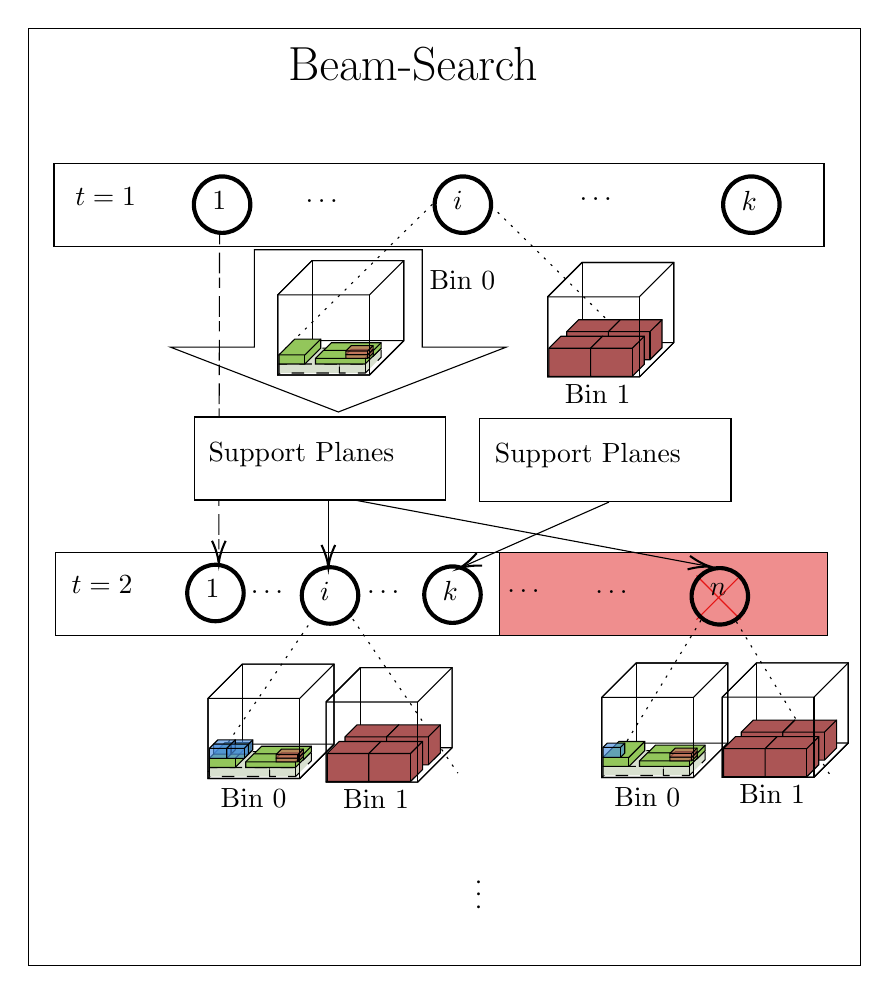
\begin{tikzpicture}[x=0.75pt,y=0.75pt,yscale=-1,xscale=1]
%uncomment if require: \path (0,540); %set diagram left start at 0, and has height of 540

%Right Arrow [id:dp8337745536636388] 
\draw   (281.86,136.75) -- (281.86,183.64) -- (322.31,183.64) -- (241.41,214.89) -- (160.5,183.64) -- (200.95,183.64) -- (200.95,136.75) -- cycle ;
%Straight Lines [id:da78157118634077] 
\draw  [dash pattern={on 3.75pt off 3pt on 7.5pt off 1.5pt}]  (184.2,129.1) -- (183.81,285.9) ;
\draw [shift={(183.8,287.9)}, rotate = 270.14] [color={rgb, 255:red, 0; green, 0; blue, 0 }  ][line width=0.75]    (10.93,-3.29) .. controls (6.95,-1.4) and (3.31,-0.3) .. (0,0) .. controls (3.31,0.3) and (6.95,1.4) .. (10.93,3.29)   ;
%Shape: Cube [id:dp22610144404804344] 
\draw   (272.94,180.54) -- (256.4,197.09) -- (212.23,197.09) -- (212.23,158.49) -- (228.77,141.94) -- (272.94,141.94) -- cycle ; \draw   (212.23,197.09) -- (228.77,180.54) -- (272.94,180.54) ; \draw   (228.77,180.54) -- (228.77,141.94) ;
%Shape: Rectangle [id:dp3675398368494672] 
\draw   (92,30) -- (493,30) -- (493,481.75) -- (92,481.75) -- cycle ;
%Shape: Rectangle [id:dp3872816319657796] 
\draw   (104.4,95) -- (475.4,95) -- (475.4,135) -- (104.4,135) -- cycle ;
%Straight Lines [id:da16266893569729468] 
\draw  [dash pattern={on 0.84pt off 2.51pt}]  (286.71,114.86) -- (211,189.14) ;
%Straight Lines [id:da2739363742069437] 
\draw  [dash pattern={on 0.84pt off 2.51pt}]  (315,115.5) -- (390.43,189.71) ;

%Shape: Cube [id:dp06723731454771065] 
\draw   (403,181.46) -- (386.46,198) -- (342.29,198) -- (342.29,159.4) -- (358.83,142.86) -- (403,142.86) -- cycle ; \draw   (342.29,198) -- (358.83,181.46) -- (403,181.46) ; \draw   (358.83,181.46) -- (358.83,142.86) ;
%Shape: Cube [id:dp9540002545180426] 
\draw  [fill={rgb, 255:red, 171; green, 85; blue, 85 }  ,fill opacity=1 ] (351.43,176.21) -- (357.21,170.43) -- (377.29,170.43) -- (377.29,183.93) -- (371.5,189.71) -- (351.43,189.71) -- cycle ; \draw   (377.29,170.43) -- (371.5,176.21) -- (351.43,176.21) ; \draw   (371.5,176.21) -- (371.5,189.71) ;
%Shape: Cube [id:dp4858900723039008] 
\draw  [fill={rgb, 255:red, 171; green, 85; blue, 85 }  ,fill opacity=1 ] (371.5,176.21) -- (377.29,170.43) -- (397.36,170.43) -- (397.36,183.93) -- (391.57,189.71) -- (371.5,189.71) -- cycle ; \draw   (397.36,170.43) -- (391.57,176.21) -- (371.5,176.21) ; \draw   (391.57,176.21) -- (391.57,189.71) ;
%Shape: Cube [id:dp37688563395090247] 
\draw  [fill={rgb, 255:red, 171; green, 85; blue, 85 }  ,fill opacity=1 ] (342.86,184.21) -- (348.64,178.43) -- (368.71,178.43) -- (368.71,191.93) -- (362.93,197.71) -- (342.86,197.71) -- cycle ; \draw   (368.71,178.43) -- (362.93,184.21) -- (342.86,184.21) ; \draw   (362.93,184.21) -- (362.93,197.71) ;
%Shape: Cube [id:dp29304074255321133] 
\draw  [fill={rgb, 255:red, 171; green, 85; blue, 85 }  ,fill opacity=1 ] (362.93,184.21) -- (368.71,178.43) -- (388.79,178.43) -- (388.79,191.93) -- (383,197.71) -- (362.93,197.71) -- cycle ; \draw   (388.79,178.43) -- (383,184.21) -- (362.93,184.21) ; \draw   (383,184.21) -- (383,197.71) ;
%Shape: Cube [id:dp012588700852047996] 
\draw   (342.29,159.4) -- (358.83,142.86) -- (403,142.86) -- (403,181.46) -- (386.46,198) -- (342.29,198) -- cycle ; \draw   (403,142.86) -- (386.46,159.4) -- (342.29,159.4) ; \draw   (386.46,159.4) -- (386.46,198) ;
%Shape: Cube [id:dp23988070590283161] 
\draw  [fill={rgb, 255:red, 216; green, 224; blue, 207 }  ,fill opacity=1 ][dash pattern={on 4.5pt off 4.5pt}] (212.84,191.76) -- (220.46,184.14) -- (249.52,184.14) -- (249.52,188.52) -- (241.9,196.13) -- (212.84,196.13) -- cycle ; \draw  [dash pattern={on 4.5pt off 4.5pt}] (249.52,184.14) -- (241.9,191.76) -- (212.84,191.76) ; \draw  [dash pattern={on 4.5pt off 4.5pt}] (241.9,191.76) -- (241.9,196.13) ;
%Shape: Cube [id:dp09035733009605551] 
\draw  [fill={rgb, 255:red, 216; green, 224; blue, 207 }  ,fill opacity=1 ][dash pattern={on 4.5pt off 4.5pt}] (241.9,191.76) -- (249.52,184.14) -- (262.04,184.14) -- (262.04,188.52) -- (254.42,196.13) -- (241.9,196.13) -- cycle ; \draw  [dash pattern={on 4.5pt off 4.5pt}] (262.04,184.14) -- (254.42,191.76) -- (241.9,191.76) ; \draw  [dash pattern={on 4.5pt off 4.5pt}] (254.42,191.76) -- (254.42,196.13) ;
%Shape: Cube [id:dp21044320148528428] 
\draw  [fill={rgb, 255:red, 147; green, 198; blue, 91 }  ,fill opacity=1 ] (212.84,187.39) -- (220.46,179.77) -- (232.93,179.77) -- (232.93,184.14) -- (225.31,191.76) -- (212.84,191.76) -- cycle ; \draw   (232.93,179.77) -- (225.31,187.39) -- (212.84,187.39) ; \draw   (225.31,187.39) -- (225.31,191.76) ;
%Shape: Cube [id:dp2634805119323166] 
\draw  [fill={rgb, 255:red, 147; green, 198; blue, 91 }  ,fill opacity=1 ] (234.29,185.34) -- (238.1,181.53) -- (262.04,181.53) -- (262.04,184.17) -- (258.22,187.99) -- (234.29,187.99) -- cycle ; \draw   (262.04,181.53) -- (258.22,185.34) -- (234.29,185.34) ; \draw   (258.22,185.34) -- (258.22,187.99) ;
%Shape: Cube [id:dp5335177162875748] 
\draw  [fill={rgb, 255:red, 147; green, 198; blue, 91 }  ,fill opacity=1 ] (230.41,189.08) -- (234.29,185.21) -- (258.16,185.21) -- (258.16,187.89) -- (254.29,191.76) -- (230.41,191.76) -- cycle ; \draw   (258.16,185.21) -- (254.29,189.08) -- (230.41,189.08) ; \draw   (254.29,189.08) -- (254.29,191.76) ;
%Shape: Cube [id:dp6236494259647203] 
\draw  [fill={rgb, 255:red, 198; green, 110; blue, 91 }  ,fill opacity=0.69 ] (245.05,187.29) -- (247.63,184.71) -- (258.16,184.71) -- (258.16,186.5) -- (255.58,189.08) -- (245.05,189.08) -- cycle ; \draw   (258.16,184.71) -- (255.58,187.29) -- (245.05,187.29) ; \draw   (255.58,187.29) -- (255.58,189.08) ;
%Shape: Cube [id:dp9516088630040508] 
\draw  [fill={rgb, 255:red, 198; green, 110; blue, 91 }  ,fill opacity=0.69 ] (245.05,185.5) -- (247.63,182.92) -- (258.16,182.92) -- (258.16,184.71) -- (255.58,187.29) -- (245.05,187.29) -- cycle ; \draw   (258.16,182.92) -- (255.58,185.5) -- (245.05,185.5) ; \draw   (255.58,185.5) -- (255.58,187.29) ;
%Shape: Cube [id:dp022246373009996434] 
\draw   (212.23,158.49) -- (228.77,141.94) -- (272.94,141.94) -- (272.94,180.54) -- (256.4,197.09) -- (212.23,197.09) -- cycle ; \draw   (272.94,141.94) -- (256.4,158.49) -- (212.23,158.49) ; \draw   (256.4,158.49) -- (256.4,197.09) ;
%Shape: Rectangle [id:dp6604290999676096] 
\draw  [fill={rgb, 255:red, 255; green, 255; blue, 255 }  ,fill opacity=1 ] (172,217.3) -- (293,217.3) -- (293,257.3) -- (172,257.3) -- cycle ;
%Shape: Rectangle [id:dp10394734829371921] 
\draw   (309.6,218.1) -- (430.6,218.1) -- (430.6,258.1) -- (309.6,258.1) -- cycle ;
%Shape: Rectangle [id:dp3884482964100383] 
\draw   (105.2,282.6) -- (476.2,282.6) -- (476.2,322.6) -- (105.2,322.6) -- cycle ;
%Shape: Rectangle [id:dp4662670618125976] 
\draw  [fill={rgb, 255:red, 239; green, 142; blue, 142 }  ,fill opacity=1 ] (319.2,282.5) -- (477,282.5) -- (477,322.5) -- (319.2,322.5) -- cycle ;
\draw  [color={rgb, 255:red, 229; green, 21; blue, 21 }  ,draw opacity=1 ] (413.99,293.69) -- (435.21,314.91)(435.21,293.69) -- (413.99,314.91) ;
%Straight Lines [id:da9423844633177114] 
\draw    (236.6,257.9) -- (236.6,287.9) ;
\draw [shift={(236.6,289.9)}, rotate = 270] [color={rgb, 255:red, 0; green, 0; blue, 0 }  ][line width=0.75]    (10.93,-3.29) .. controls (6.95,-1.4) and (3.31,-0.3) .. (0,0) .. controls (3.31,0.3) and (6.95,1.4) .. (10.93,3.29)   ;
%Straight Lines [id:da8187100513502555] 
\draw    (250.2,257.5) -- (419.03,289.13) ;
\draw [shift={(421,289.5)}, rotate = 190.61] [color={rgb, 255:red, 0; green, 0; blue, 0 }  ][line width=0.75]    (10.93,-3.29) .. controls (6.95,-1.4) and (3.31,-0.3) .. (0,0) .. controls (3.31,0.3) and (6.95,1.4) .. (10.93,3.29)   ;
%Straight Lines [id:da5112317799583161] 
\draw    (371.8,258.3) -- (301.23,289.49) ;
\draw [shift={(299.4,290.3)}, rotate = 336.16] [color={rgb, 255:red, 0; green, 0; blue, 0 }  ][line width=0.75]    (10.93,-3.29) .. controls (6.95,-1.4) and (3.31,-0.3) .. (0,0) .. controls (3.31,0.3) and (6.95,1.4) .. (10.93,3.29)   ;
%Shape: Cube [id:dp3098593802776677] 
\draw   (239.34,374.94) -- (222.8,391.49) -- (178.63,391.49) -- (178.63,352.89) -- (195.17,336.34) -- (239.34,336.34) -- cycle ; \draw   (178.63,391.49) -- (195.17,374.94) -- (239.34,374.94) ; \draw   (195.17,374.94) -- (195.17,336.34) ;
%Straight Lines [id:da052289940556063064] 
\draw  [dash pattern={on 0.84pt off 2.51pt}]  (229.41,314.06) -- (178.6,388.34) ;
%Straight Lines [id:da7979737763702788] 
\draw  [dash pattern={on 0.84pt off 2.51pt}]  (248.39,314.7) -- (299,388.91) ;

%Shape: Cube [id:dp563730868795463] 
\draw   (296.2,376.66) -- (279.66,393.2) -- (235.49,393.2) -- (235.49,354.6) -- (252.03,338.06) -- (296.2,338.06) -- cycle ; \draw   (235.49,393.2) -- (252.03,376.66) -- (296.2,376.66) ; \draw   (252.03,376.66) -- (252.03,338.06) ;
%Shape: Cube [id:dp6842297170502628] 
\draw  [fill={rgb, 255:red, 171; green, 85; blue, 85 }  ,fill opacity=1 ] (244.63,371.41) -- (250.41,365.63) -- (270.49,365.63) -- (270.49,379.13) -- (264.7,384.91) -- (244.63,384.91) -- cycle ; \draw   (270.49,365.63) -- (264.7,371.41) -- (244.63,371.41) ; \draw   (264.7,371.41) -- (264.7,384.91) ;
%Shape: Cube [id:dp36117121382423767] 
\draw  [fill={rgb, 255:red, 171; green, 85; blue, 85 }  ,fill opacity=1 ] (264.7,371.41) -- (270.49,365.63) -- (290.56,365.63) -- (290.56,379.13) -- (284.77,384.91) -- (264.7,384.91) -- cycle ; \draw   (290.56,365.63) -- (284.77,371.41) -- (264.7,371.41) ; \draw   (284.77,371.41) -- (284.77,384.91) ;
%Shape: Cube [id:dp5567622602150145] 
\draw  [fill={rgb, 255:red, 171; green, 85; blue, 85 }  ,fill opacity=1 ] (236.06,379.41) -- (241.84,373.63) -- (261.91,373.63) -- (261.91,387.13) -- (256.13,392.91) -- (236.06,392.91) -- cycle ; \draw   (261.91,373.63) -- (256.13,379.41) -- (236.06,379.41) ; \draw   (256.13,379.41) -- (256.13,392.91) ;
%Shape: Cube [id:dp9251910046018463] 
\draw  [fill={rgb, 255:red, 171; green, 85; blue, 85 }  ,fill opacity=1 ] (256.13,379.41) -- (261.91,373.63) -- (281.99,373.63) -- (281.99,387.13) -- (276.2,392.91) -- (256.13,392.91) -- cycle ; \draw   (281.99,373.63) -- (276.2,379.41) -- (256.13,379.41) ; \draw   (276.2,379.41) -- (276.2,392.91) ;
%Shape: Cube [id:dp97100963444055] 
\draw   (235.49,354.6) -- (252.03,338.06) -- (296.2,338.06) -- (296.2,376.66) -- (279.66,393.2) -- (235.49,393.2) -- cycle ; \draw   (296.2,338.06) -- (279.66,354.6) -- (235.49,354.6) ; \draw   (279.66,354.6) -- (279.66,393.2) ;
%Shape: Cube [id:dp3314229379764526] 
\draw  [fill={rgb, 255:red, 216; green, 224; blue, 207 }  ,fill opacity=1 ][dash pattern={on 4.5pt off 4.5pt}] (179.24,386.16) -- (186.86,378.54) -- (215.92,378.54) -- (215.92,382.92) -- (208.3,390.53) -- (179.24,390.53) -- cycle ; \draw  [dash pattern={on 4.5pt off 4.5pt}] (215.92,378.54) -- (208.3,386.16) -- (179.24,386.16) ; \draw  [dash pattern={on 4.5pt off 4.5pt}] (208.3,386.16) -- (208.3,390.53) ;
%Shape: Cube [id:dp4227409563137523] 
\draw  [fill={rgb, 255:red, 216; green, 224; blue, 207 }  ,fill opacity=1 ][dash pattern={on 4.5pt off 4.5pt}] (208.3,386.16) -- (215.92,378.54) -- (228.44,378.54) -- (228.44,382.92) -- (220.82,390.53) -- (208.3,390.53) -- cycle ; \draw  [dash pattern={on 4.5pt off 4.5pt}] (228.44,378.54) -- (220.82,386.16) -- (208.3,386.16) ; \draw  [dash pattern={on 4.5pt off 4.5pt}] (220.82,386.16) -- (220.82,390.53) ;
%Shape: Cube [id:dp9493780297339603] 
\draw  [fill={rgb, 255:red, 147; green, 198; blue, 91 }  ,fill opacity=1 ] (179.24,381.79) -- (186.86,374.17) -- (199.33,374.17) -- (199.33,378.54) -- (191.71,386.16) -- (179.24,386.16) -- cycle ; \draw   (199.33,374.17) -- (191.71,381.79) -- (179.24,381.79) ; \draw   (191.71,381.79) -- (191.71,386.16) ;
%Shape: Cube [id:dp20210982349003004] 
\draw  [fill={rgb, 255:red, 147; green, 198; blue, 91 }  ,fill opacity=1 ] (200.69,379.74) -- (204.5,375.93) -- (228.44,375.93) -- (228.44,378.57) -- (224.62,382.39) -- (200.69,382.39) -- cycle ; \draw   (228.44,375.93) -- (224.62,379.74) -- (200.69,379.74) ; \draw   (224.62,379.74) -- (224.62,382.39) ;
%Shape: Cube [id:dp6451220456842981] 
\draw  [fill={rgb, 255:red, 147; green, 198; blue, 91 }  ,fill opacity=1 ] (196.81,383.48) -- (200.69,379.61) -- (224.56,379.61) -- (224.56,382.29) -- (220.69,386.16) -- (196.81,386.16) -- cycle ; \draw   (224.56,379.61) -- (220.69,383.48) -- (196.81,383.48) ; \draw   (220.69,383.48) -- (220.69,386.16) ;
%Shape: Cube [id:dp3910721600427305] 
\draw  [fill={rgb, 255:red, 198; green, 110; blue, 91 }  ,fill opacity=0.69 ] (211.45,381.69) -- (214.03,379.11) -- (224.56,379.11) -- (224.56,380.9) -- (221.98,383.48) -- (211.45,383.48) -- cycle ; \draw   (224.56,379.11) -- (221.98,381.69) -- (211.45,381.69) ; \draw   (221.98,381.69) -- (221.98,383.48) ;
%Shape: Cube [id:dp23309754303051422] 
\draw  [fill={rgb, 255:red, 198; green, 110; blue, 91 }  ,fill opacity=0.69 ] (211.45,379.9) -- (214.03,377.32) -- (224.56,377.32) -- (224.56,379.11) -- (221.98,381.69) -- (211.45,381.69) -- cycle ; \draw   (224.56,377.32) -- (221.98,379.9) -- (211.45,379.9) ; \draw   (221.98,379.9) -- (221.98,381.69) ;
%Shape: Cube [id:dp4655482842473665] 
\draw   (178.63,352.89) -- (195.17,336.34) -- (239.34,336.34) -- (239.34,374.94) -- (222.8,391.49) -- (178.63,391.49) -- cycle ; \draw   (239.34,336.34) -- (222.8,352.89) -- (178.63,352.89) ; \draw   (222.8,352.89) -- (222.8,391.49) ;
%Shape: Cube [id:dp4152358812705026] 
\draw   (429.04,374.44) -- (412.5,390.99) -- (368.33,390.99) -- (368.33,352.39) -- (384.87,335.84) -- (429.04,335.84) -- cycle ; \draw   (368.33,390.99) -- (384.87,374.44) -- (429.04,374.44) ; \draw   (384.87,374.44) -- (384.87,335.84) ;
%Straight Lines [id:da6929539156017857] 
\draw  [dash pattern={on 0.84pt off 2.51pt}]  (416.13,315.26) -- (370.6,389.54) ;
%Straight Lines [id:da2520104054773419] 
\draw  [dash pattern={on 0.84pt off 2.51pt}]  (433.14,315.9) -- (478.5,390.11) ;

%Shape: Cube [id:dp30742448269234246] 
\draw   (487.1,374.36) -- (470.56,390.9) -- (426.39,390.9) -- (426.39,352.3) -- (442.93,335.76) -- (487.1,335.76) -- cycle ; \draw   (426.39,390.9) -- (442.93,374.36) -- (487.1,374.36) ; \draw   (442.93,374.36) -- (442.93,335.76) ;
%Shape: Cube [id:dp5547181392678717] 
\draw  [fill={rgb, 255:red, 171; green, 85; blue, 85 }  ,fill opacity=1 ] (435.53,369.11) -- (441.31,363.33) -- (461.39,363.33) -- (461.39,376.83) -- (455.6,382.61) -- (435.53,382.61) -- cycle ; \draw   (461.39,363.33) -- (455.6,369.11) -- (435.53,369.11) ; \draw   (455.6,369.11) -- (455.6,382.61) ;
%Shape: Cube [id:dp7714989563411607] 
\draw  [fill={rgb, 255:red, 171; green, 85; blue, 85 }  ,fill opacity=1 ] (455.6,369.11) -- (461.39,363.33) -- (481.46,363.33) -- (481.46,376.83) -- (475.67,382.61) -- (455.6,382.61) -- cycle ; \draw   (481.46,363.33) -- (475.67,369.11) -- (455.6,369.11) ; \draw   (475.67,369.11) -- (475.67,382.61) ;
%Shape: Cube [id:dp6802562603958051] 
\draw  [fill={rgb, 255:red, 171; green, 85; blue, 85 }  ,fill opacity=1 ] (426.96,377.11) -- (432.74,371.33) -- (452.81,371.33) -- (452.81,384.83) -- (447.03,390.61) -- (426.96,390.61) -- cycle ; \draw   (452.81,371.33) -- (447.03,377.11) -- (426.96,377.11) ; \draw   (447.03,377.11) -- (447.03,390.61) ;
%Shape: Cube [id:dp3575223135416413] 
\draw  [fill={rgb, 255:red, 171; green, 85; blue, 85 }  ,fill opacity=1 ] (447.03,377.11) -- (452.81,371.33) -- (472.89,371.33) -- (472.89,384.83) -- (467.1,390.61) -- (447.03,390.61) -- cycle ; \draw   (472.89,371.33) -- (467.1,377.11) -- (447.03,377.11) ; \draw   (467.1,377.11) -- (467.1,390.61) ;
%Shape: Cube [id:dp04583492087348129] 
\draw   (426.39,352.3) -- (442.93,335.76) -- (487.1,335.76) -- (487.1,374.36) -- (470.56,390.9) -- (426.39,390.9) -- cycle ; \draw   (487.1,335.76) -- (470.56,352.3) -- (426.39,352.3) ; \draw   (470.56,352.3) -- (470.56,390.9) ;
%Shape: Cube [id:dp22648598314600765] 
\draw  [fill={rgb, 255:red, 216; green, 224; blue, 207 }  ,fill opacity=1 ][dash pattern={on 4.5pt off 4.5pt}] (368.94,385.66) -- (376.56,378.04) -- (405.62,378.04) -- (405.62,382.42) -- (398,390.03) -- (368.94,390.03) -- cycle ; \draw  [dash pattern={on 4.5pt off 4.5pt}] (405.62,378.04) -- (398,385.66) -- (368.94,385.66) ; \draw  [dash pattern={on 4.5pt off 4.5pt}] (398,385.66) -- (398,390.03) ;
%Shape: Cube [id:dp11910803660750402] 
\draw  [fill={rgb, 255:red, 216; green, 224; blue, 207 }  ,fill opacity=1 ][dash pattern={on 4.5pt off 4.5pt}] (398,385.66) -- (405.62,378.04) -- (418.14,378.04) -- (418.14,382.42) -- (410.52,390.03) -- (398,390.03) -- cycle ; \draw  [dash pattern={on 4.5pt off 4.5pt}] (418.14,378.04) -- (410.52,385.66) -- (398,385.66) ; \draw  [dash pattern={on 4.5pt off 4.5pt}] (410.52,385.66) -- (410.52,390.03) ;
%Shape: Cube [id:dp03436669328315789] 
\draw  [fill={rgb, 255:red, 147; green, 198; blue, 91 }  ,fill opacity=1 ] (368.94,381.29) -- (376.56,373.67) -- (389.03,373.67) -- (389.03,378.04) -- (381.41,385.66) -- (368.94,385.66) -- cycle ; \draw   (389.03,373.67) -- (381.41,381.29) -- (368.94,381.29) ; \draw   (381.41,381.29) -- (381.41,385.66) ;
%Shape: Cube [id:dp3001366964737242] 
\draw  [fill={rgb, 255:red, 147; green, 198; blue, 91 }  ,fill opacity=1 ] (390.39,379.24) -- (394.2,375.43) -- (418.14,375.43) -- (418.14,378.07) -- (414.32,381.89) -- (390.39,381.89) -- cycle ; \draw   (418.14,375.43) -- (414.32,379.24) -- (390.39,379.24) ; \draw   (414.32,379.24) -- (414.32,381.89) ;
%Shape: Cube [id:dp9791091368910745] 
\draw  [fill={rgb, 255:red, 147; green, 198; blue, 91 }  ,fill opacity=1 ] (386.51,382.98) -- (390.39,379.11) -- (414.26,379.11) -- (414.26,381.79) -- (410.39,385.66) -- (386.51,385.66) -- cycle ; \draw   (414.26,379.11) -- (410.39,382.98) -- (386.51,382.98) ; \draw   (410.39,382.98) -- (410.39,385.66) ;
%Shape: Cube [id:dp5345838256134253] 
\draw  [fill={rgb, 255:red, 198; green, 110; blue, 91 }  ,fill opacity=0.69 ] (401.15,381.19) -- (403.73,378.61) -- (414.26,378.61) -- (414.26,380.4) -- (411.68,382.98) -- (401.15,382.98) -- cycle ; \draw   (414.26,378.61) -- (411.68,381.19) -- (401.15,381.19) ; \draw   (411.68,381.19) -- (411.68,382.98) ;
%Shape: Cube [id:dp8233627388074675] 
\draw  [fill={rgb, 255:red, 74; green, 144; blue, 226 }  ,fill opacity=0.66 ] (368.94,376.49) -- (370.99,374.44) -- (379.4,374.44) -- (379.4,379.24) -- (377.34,381.29) -- (368.94,381.29) -- cycle ; \draw   (379.4,374.44) -- (377.34,376.49) -- (368.94,376.49) ; \draw   (377.34,376.49) -- (377.34,381.29) ;
%Shape: Cube [id:dp3945702568476691] 
\draw  [fill={rgb, 255:red, 198; green, 110; blue, 91 }  ,fill opacity=0.69 ] (401.15,379.4) -- (403.73,376.82) -- (414.26,376.82) -- (414.26,378.61) -- (411.68,381.19) -- (401.15,381.19) -- cycle ; \draw   (414.26,376.82) -- (411.68,379.4) -- (401.15,379.4) ; \draw   (411.68,379.4) -- (411.68,381.19) ;
%Shape: Cube [id:dp8251331839204266] 
\draw   (368.33,352.39) -- (384.87,335.84) -- (429.04,335.84) -- (429.04,374.44) -- (412.5,390.99) -- (368.33,390.99) -- cycle ; \draw   (429.04,335.84) -- (412.5,352.39) -- (368.33,352.39) ; \draw   (412.5,352.39) -- (412.5,390.99) ;
%Shape: Cube [id:dp2708464120930435] 
\draw  [fill={rgb, 255:red, 74; green, 144; blue, 226 }  ,fill opacity=0.66 ] (189.7,374.94) -- (191.75,372.88) -- (200.16,372.88) -- (200.16,377.68) -- (198.1,379.74) -- (189.7,379.74) -- cycle ; \draw   (200.16,372.88) -- (198.1,374.94) -- (189.7,374.94) ; \draw   (198.1,374.94) -- (198.1,379.74) ;
%Shape: Cube [id:dp15483932168959624] 
\draw  [fill={rgb, 255:red, 74; green, 144; blue, 226 }  ,fill opacity=0.66 ] (181.29,374.94) -- (183.35,372.88) -- (191.75,372.88) -- (191.75,377.68) -- (189.7,379.74) -- (181.29,379.74) -- cycle ; \draw   (191.75,372.88) -- (189.7,374.94) -- (181.29,374.94) ; \draw   (189.7,374.94) -- (189.7,379.74) ;
%Shape: Cube [id:dp5792684196727304] 
\draw  [fill={rgb, 255:red, 74; green, 144; blue, 226 }  ,fill opacity=0.66 ] (179.24,376.99) -- (181.29,374.94) -- (189.7,374.94) -- (189.7,379.74) -- (187.64,381.79) -- (179.24,381.79) -- cycle ; \draw   (189.7,374.94) -- (187.64,376.99) -- (179.24,376.99) ; \draw   (187.64,376.99) -- (187.64,381.79) ;
%Shape: Cube [id:dp6982160774307449] 
\draw  [fill={rgb, 255:red, 74; green, 144; blue, 226 }  ,fill opacity=0.66 ] (187.64,376.99) -- (189.7,374.94) -- (198.1,374.94) -- (198.1,379.74) -- (196.04,381.79) -- (187.64,381.79) -- cycle ; \draw   (198.1,374.94) -- (196.04,376.99) -- (187.64,376.99) ; \draw   (196.04,376.99) -- (196.04,381.79) ;

% Text Node
\draw (216,38) node [anchor=north west][inner sep=0.75pt]   [align=left] {{\LARGE Beam-Search}};
% Text Node
\draw  [line width=1.5]   (185.4, 115) circle [x radius= 13.6, y radius= 13.6]   ;
\draw (179.4,107.4) node [anchor=north west][inner sep=0.75pt]    {$1$};
% Text Node
\draw (113.4,105.4) node [anchor=north west][inner sep=0.75pt]    {$t=1$};
% Text Node
\draw  [line width=1.5]   (301.4, 115) circle [x radius= 13.6, y radius= 13.6]   ;
\draw (295.4,107.4) node [anchor=north west][inner sep=0.75pt]    {$i$};
% Text Node
\draw  [line width=1.5]   (440.4, 115) circle [x radius= 13.6, y radius= 13.6]   ;
\draw (434.4,107.4) node [anchor=north west][inner sep=0.75pt]    {$k$};
% Text Node
\draw (224.4,111.4) node [anchor=north west][inner sep=0.75pt]    {$\dotsc $};
% Text Node
\draw (356.4,110.4) node [anchor=north west][inner sep=0.75pt]    {$\dotsc $};
% Text Node
\draw (284.09,145.3) node [anchor=north west][inner sep=0.75pt]   [align=left] {Bin 0};
% Text Node
\draw (349.26,200.23) node [anchor=north west][inner sep=0.75pt]   [align=left] {Bin 1};
% Text Node
\draw (177.6,228.1) node [anchor=north west][inner sep=0.75pt]   [align=left] {Support Planes};
% Text Node
\draw (315.6,228.5) node [anchor=north west][inner sep=0.75pt]   [align=left] {Support Planes};
% Text Node
\draw  [line width=1.5]   (182.2, 302.1) circle [x radius= 13.6, y radius= 13.6]   ;
\draw (176.2,294.5) node [anchor=north west][inner sep=0.75pt]    {$1$};
% Text Node
\draw (111.7,292.5) node [anchor=north west][inner sep=0.75pt]    {$t=2$};
% Text Node
\draw  [line width=1.5]   (237.4, 303.3) circle [x radius= 13.6, y radius= 13.6]   ;
\draw (231.4,295.7) node [anchor=north west][inner sep=0.75pt]    {$i$};
% Text Node
\draw  [line width=1.5]   (296.4, 302.9) circle [x radius= 13.6, y radius= 13.6]   ;
\draw (290.4,295.3) node [anchor=north west][inner sep=0.75pt]    {$k$};
% Text Node
\draw (198,299.7) node [anchor=north west][inner sep=0.75pt]    {$\dotsc $};
% Text Node
\draw (254,299.5) node [anchor=north west][inner sep=0.75pt]    {$\dotsc $};
% Text Node
\draw (321.6,299.1) node [anchor=north west][inner sep=0.75pt]    {$\dotsc $};
% Text Node
\draw  [line width=1.5]   (425.2, 303.7) circle [x radius= 13.6, y radius= 13.6]   ;
\draw (419.2,296.1) node [anchor=north west][inner sep=0.75pt]    {$n$};
% Text Node
\draw (364,299.5) node [anchor=north west][inner sep=0.75pt]    {$\dotsc $};
% Text Node
\draw (310.95,438.37) node [anchor=north west][inner sep=0.75pt]  [rotate=-89.78]  {$\dotsc $};
% Text Node
\draw (183.49,395.2) node [anchor=north west][inner sep=0.75pt]   [align=left] {Bin 0};
% Text Node
\draw (242.46,395.43) node [anchor=north west][inner sep=0.75pt]   [align=left] {Bin 1};
% Text Node
\draw (373.19,394.7) node [anchor=north west][inner sep=0.75pt]   [align=left] {Bin 0};
% Text Node
\draw (433.36,393.13) node [anchor=north west][inner sep=0.75pt]   [align=left] {Bin 1};


\end{tikzpicture}

            }
            \caption{Conceptual representation of the proposed heuristic}
            \label{fig:heur_scheme}
        \end{figure}
    \end{frame}
    \begin{frame}{Support Plane}
    \end{frame}
    \begin{frame}{Beam Search}
    \end{frame}
    \begin{frame}{Optimizations}
    \end{frame}

    \section{Conclusions}

    \begin{frame}{Computational Experiments}
    \end{frame}

    \begin{frame}{Results \& Future Developments}
    \end{frame}
\end{document}